% Options for packages loaded elsewhere
\PassOptionsToPackage{unicode}{hyperref}
\PassOptionsToPackage{hyphens}{url}
%
\documentclass[
  11pt,
  a4paper]{article}
\usepackage{mathptmx}
\usepackage{setspace}
\usepackage{amssymb,amsmath}
\usepackage{ifxetex,ifluatex}
\ifnum 0\ifxetex 1\fi\ifluatex 1\fi=0 % if pdftex
  \usepackage[T1]{fontenc}
  \usepackage[utf8]{inputenc}
  \usepackage{textcomp} % provide euro and other symbols
\else % if luatex or xetex
  \usepackage{unicode-math}
  \defaultfontfeatures{Scale=MatchLowercase}
  \defaultfontfeatures[\rmfamily]{Ligatures=TeX,Scale=1}
\fi
% Use upquote if available, for straight quotes in verbatim environments
\IfFileExists{upquote.sty}{\usepackage{upquote}}{}
\IfFileExists{microtype.sty}{% use microtype if available
  \usepackage[]{microtype}
  \UseMicrotypeSet[protrusion]{basicmath} % disable protrusion for tt fonts
}{}
\makeatletter
\@ifundefined{KOMAClassName}{% if non-KOMA class
  \IfFileExists{parskip.sty}{%
    \usepackage{parskip}
  }{% else
    \setlength{\parindent}{0pt}
    \setlength{\parskip}{6pt plus 2pt minus 1pt}}
}{% if KOMA class
  \KOMAoptions{parskip=half}}
\makeatother
\usepackage{xcolor}
\IfFileExists{xurl.sty}{\usepackage{xurl}}{} % add URL line breaks if available
\IfFileExists{bookmark.sty}{\usepackage{bookmark}}{\usepackage{hyperref}}
\hypersetup{
  pdftitle={LLM-Enhanced Disk Failure Prediction on Top of StreamDFP: System Design, Evaluation, and First-Term Progress},
  pdfauthor={Student Name: Daoyang LIU Student ID: 1155244610 Master of Science in Artificial Intelligence AIMS5790 Artificial Intelligence Project I},
  hidelinks,
  pdfcreator={LaTeX via pandoc}}
\urlstyle{same} % disable monospaced font for URLs
\usepackage[margin=1in]{geometry}
\usepackage{color}
\usepackage{fancyvrb}
\newcommand{\VerbBar}{|}
\newcommand{\VERB}{\Verb[commandchars=\\\{\}]}
\DefineVerbatimEnvironment{Highlighting}{Verbatim}{commandchars=\\\{\},fontsize=\footnotesize}
% Add ',fontsize=\small' for more characters per line
\newenvironment{Shaded}{}{}
\newcommand{\AlertTok}[1]{\textcolor[rgb]{1.00,0.00,0.00}{\textbf{#1}}}
\newcommand{\AnnotationTok}[1]{\textcolor[rgb]{0.38,0.63,0.69}{\textbf{\textit{#1}}}}
\newcommand{\AttributeTok}[1]{\textcolor[rgb]{0.49,0.56,0.16}{#1}}
\newcommand{\BaseNTok}[1]{\textcolor[rgb]{0.25,0.63,0.44}{#1}}
\newcommand{\BuiltInTok}[1]{#1}
\newcommand{\CharTok}[1]{\textcolor[rgb]{0.25,0.44,0.63}{#1}}
\newcommand{\CommentTok}[1]{\textcolor[rgb]{0.38,0.63,0.69}{\textit{#1}}}
\newcommand{\CommentVarTok}[1]{\textcolor[rgb]{0.38,0.63,0.69}{\textbf{\textit{#1}}}}
\newcommand{\ConstantTok}[1]{\textcolor[rgb]{0.53,0.00,0.00}{#1}}
\newcommand{\ControlFlowTok}[1]{\textcolor[rgb]{0.00,0.44,0.13}{\textbf{#1}}}
\newcommand{\DataTypeTok}[1]{\textcolor[rgb]{0.56,0.13,0.00}{#1}}
\newcommand{\DecValTok}[1]{\textcolor[rgb]{0.25,0.63,0.44}{#1}}
\newcommand{\DocumentationTok}[1]{\textcolor[rgb]{0.73,0.13,0.13}{\textit{#1}}}
\newcommand{\ErrorTok}[1]{\textcolor[rgb]{1.00,0.00,0.00}{\textbf{#1}}}
\newcommand{\ExtensionTok}[1]{#1}
\newcommand{\FloatTok}[1]{\textcolor[rgb]{0.25,0.63,0.44}{#1}}
\newcommand{\FunctionTok}[1]{\textcolor[rgb]{0.02,0.16,0.49}{#1}}
\newcommand{\ImportTok}[1]{#1}
\newcommand{\InformationTok}[1]{\textcolor[rgb]{0.38,0.63,0.69}{\textbf{\textit{#1}}}}
\newcommand{\KeywordTok}[1]{\textcolor[rgb]{0.00,0.44,0.13}{\textbf{#1}}}
\newcommand{\NormalTok}[1]{#1}
\newcommand{\OperatorTok}[1]{\textcolor[rgb]{0.40,0.40,0.40}{#1}}
\newcommand{\OtherTok}[1]{\textcolor[rgb]{0.00,0.44,0.13}{#1}}
\newcommand{\PreprocessorTok}[1]{\textcolor[rgb]{0.74,0.48,0.00}{#1}}
\newcommand{\RegionMarkerTok}[1]{#1}
\newcommand{\SpecialCharTok}[1]{\textcolor[rgb]{0.25,0.44,0.63}{#1}}
\newcommand{\SpecialStringTok}[1]{\textcolor[rgb]{0.73,0.40,0.53}{#1}}
\newcommand{\StringTok}[1]{\textcolor[rgb]{0.25,0.44,0.63}{#1}}
\newcommand{\VariableTok}[1]{\textcolor[rgb]{0.10,0.09,0.49}{#1}}
\newcommand{\VerbatimStringTok}[1]{\textcolor[rgb]{0.25,0.44,0.63}{#1}}
\newcommand{\WarningTok}[1]{\textcolor[rgb]{0.38,0.63,0.69}{\textbf{\textit{#1}}}}
\usepackage{longtable,booktabs}
% Correct order of tables after \paragraph or \subparagraph
\usepackage{etoolbox}
\makeatletter
\patchcmd\longtable{\par}{\if@noskipsec\mbox{}\fi\par}{}{}
\makeatother
% Allow footnotes in longtable head/foot
\IfFileExists{footnotehyper.sty}{\usepackage{footnotehyper}}{\usepackage{footnote}}
\makesavenoteenv{longtable}
\usepackage{graphicx}
\makeatletter
\def\maxwidth{\ifdim\Gin@nat@width>\linewidth\linewidth\else\Gin@nat@width\fi}
\def\maxheight{\ifdim\Gin@nat@height>\textheight\textheight\else\Gin@nat@height\fi}
\makeatother
% Scale images if necessary, so that they will not overflow the page
% margins by default, and it is still possible to overwrite the defaults
% using explicit options in \includegraphics[width, height, ...]{}
\setkeys{Gin}{width=\maxwidth,height=\maxheight,keepaspectratio}
% Set default figure placement to htbp
\makeatletter
\def\fps@figure{htbp}
\makeatother
\setlength{\emergencystretch}{3em} % prevent overfull lines
\providecommand{\tightlist}{%
  \setlength{\itemsep}{0pt}\setlength{\parskip}{0pt}}
\setcounter{secnumdepth}{-\maxdimen} % remove section numbering
\usepackage{caption}
\usepackage{float}
\usepackage{fancyhdr}
\usepackage{titlesec}
\usepackage{enumitem}
\captionsetup{font=small,labelfont=bf,skip=4pt}
\setlist{itemsep=0.3em, topsep=0.3em}
\titleformat{\section}{\Large\bfseries}{}{0pt}{}
\titleformat{\subsection}{\large\bfseries}{}{0pt}{}
\titleformat{\subsubsection}{\normalsize\bfseries}{}{0pt}{}
\titlespacing*{\section}{0pt}{1.0em}{0.4em}
\titlespacing*{\subsection}{0pt}{0.8em}{0.3em}
\titlespacing*{\subsubsection}{0pt}{0.6em}{0.25em}
\pagestyle{fancy}
\fancyhf{}
\fancyfoot[C]{\thepage}
\renewcommand{\headrulewidth}{0pt}
\setlength{\headheight}{14pt}
\setlength{\textfloatsep}{10pt plus 2pt minus 2pt}
\setlength{\floatsep}{8pt plus 2pt minus 2pt}
\setlength{\intextsep}{8pt plus 2pt minus 2pt}
\setlength{\abovecaptionskip}{4pt}
\setlength{\belowcaptionskip}{0pt}
\setlength{\LTpre}{6pt}
\setlength{\LTpost}{6pt}
\AtBeginEnvironment{longtable}{\small\setlength{\tabcolsep}{4pt}\renewcommand{\arraystretch}{1.08}}
\AtEndEnvironment{longtable}{\normalsize\renewcommand{\arraystretch}{1.0}}

\title{LLM-Enhanced Disk Failure Prediction on Top of StreamDFP: System
Design, Evaluation, and First-Term Progress}
\author{Student Name: Daoyang LIU\\
Student ID: 1155244610\\
Master of Science in Artificial Intelligence\\
AIMS5790 Artificial Intelligence Project I}
\date{April 2026}

\begin{document}
\hypersetup{pageanchor=false}
\begin{titlepage}
\thispagestyle{empty}
\centering
\vspace*{1.2cm}
{\Large AIMS5790 Artificial Intelligence Project I\par}
\vspace{0.8cm}
{\large Master of Science in Artificial Intelligence\par}
\vspace{1.1cm}
{\Huge \bfseries LLM-Enhanced Disk Failure Prediction on Top of StreamDFP\par}
\vspace{0.25cm}
{\Large \bfseries System Design, Evaluation, and First-Term Progress\par}
\vfill
{\large Student Name: Daoyang LIU\par}
\vspace{0.2cm}
{\large Student ID: 1155244610\par}
\vspace{0.8cm}
{\large Faculty of Engineering\par}
{\large The Chinese University of Hong Kong\par}
\vspace{0.8cm}
{\large April 2026\par}
\end{titlepage}

\hypersetup{pageanchor=true}
\pagenumbering{roman}
{
\setcounter{tocdepth}{2}
\footnotesize
\setstretch{0.94}
\setlength{\parskip}{0pt}
\tableofcontents
}
\clearpage
\pagenumbering{arabic}
\setstretch{1.0}
\hypertarget{abstract}{%
\section{Abstract}\label{abstract}}

Disk failure prediction based on SMART telemetry remains a central
problem in storage reliability, yet most practical pipelines rely
predominantly on numerical features and therefore offer limited semantic
interpretability. This report presents an extension of StreamDFP with a
structured large-language-model enhancement layer while preserving the
original Python-Java prediction backbone. The proposed method comprises
three stages. Phase 1 converts time-windowed SMART records into
constrained textual summaries. Phase 2 performs offline semantic
extraction and maps the outputs into fixed-dimensional cache features.
Phase 3 evaluates gated feature variants under exactly the same
simulation protocol as the no-LLM baseline. The resulting framework also
incorporates disk-model-level policy selection, an onboarding branch for
new disk models, workflow wrappers, and a local workbench to strengthen
reproducibility.

The first-term results indicate that semantic enhancement is beneficial
only under selective activation rather than uniform deployment. On the
retained HDD benchmark, Qwen3-4B-Instruct-2507 enables 8 disk models
with an average Delta Recall of 18.0903 over accepted models, whereas
Qwen3.5-4B and Qwen3.5-Plus each enable 7 models with average Delta
Recall values of 19.2081 and 20.1520, respectively. For the mc1 SSD
case, once the faulty sequential sampling pipeline was repaired and
replaced with stratified\_v2, all three candidate models converged to
the same best retained configuration, achieving Recall = 100.0000, ACC =
99.5489, and Delta Recall = +2.2296 relative to the no-LLM baseline.
Overall, the evidence suggests that LLM-derived semantic signals are
most useful when they are cache-based, selectively gated, and validated
under a unified baseline protocol. The second term will therefore focus
on policy consolidation, lower-cost Phase 3 evaluation, and stronger
statistical validation.

\hypertarget{introduction}{%
\section{1. Introduction}\label{introduction}}

\hypertarget{background}{%
\subsection{1.1 Background}\label{background}}

Disk failure prediction is a long-standing problem in intelligent
storage and reliability management. In operational settings, SMART
statistics are attractive because they are inexpensive to collect,
updated continuously, and compatible with automated monitoring
pipelines. However, raw SMART features have limited semantic
expressiveness. They are useful for classification and ranking, yet they
do not directly encode higher-level causes such as media degradation,
interface instability, thermal stress, or workload-related anomalies. As
a result, it is difficult to combine predictive performance with
interpretable reasoning.

The upstream StreamDFP framework provides a strong baseline for this
problem {[}1{]}. It combines Python preprocessing with Java-based
simulation to support time-ordered learning and evaluation, making it
suitable for disk-health prediction in a streaming setting.
Nevertheless, the baseline still exhibits three practical limitations.
First, it relies primarily on numerical features and therefore lacks
explicit root-cause semantics. Second, a single enhancement strategy is
unlikely to perform equally well across all disk models. Third, as the
project evolves across Python, Java, local LLMs, API models, and
numerous shell scripts, reproducibility and operability become research
challenges in their own right.

\hypertarget{problem-statement}{%
\subsection{1.2 Problem Statement}\label{problem-statement}}

This project investigates whether LLM-extracted semantic signals can be
reinjected into the original StreamDFP prediction chain so as to improve
performance without violating the baseline evaluation protocol. The
objective is not to replace StreamDFP with an end-to-end language-based
predictor. Instead, the aim is to construct a hybrid system in which
structured semantic evidence is generated offline, compressed into
comparable numerical features, and re-evaluated through the same
training and simulation path as the no-LLM baseline.

\hypertarget{research-questions}{%
\subsection{1.3 Research Questions}\label{research-questions}}

The first-term study is organized around four research questions.

\begin{enumerate}
\def\labelenumi{\arabic{enumi}.}
\tightlist
\item
  Can SMART time-window statistics be converted into a structured
  textual representation that is suitable for constrained LLM
  extraction?
\item
  Can LLM outputs such as root causes, events, confidence, and risk
  hints be normalized into fixed-dimensional features that can be
  consumed by the original predictor?
\item
  Should LLM enhancement be applied to all disk models, or should
  activation be decided at the disk-model level under explicit guards?
\item
  How can such a hybrid Python-Java-LLM system remain reproducible and
  operable in a real research workflow?
\end{enumerate}

\hypertarget{contributions}{%
\subsection{1.4 Contributions}\label{contributions}}

The first-term contributions of the project are as follows.

\begin{enumerate}
\def\labelenumi{\arabic{enumi}.}
\tightlist
\item
  A closed-loop hybrid architecture that extends StreamDFP without
  breaking comparability with the original prediction chain.
\item
  A cache-based semantic-feature design that transforms LLM extraction
  into comparable profiles such as compact9, compact14, and full70.
\item
  A disk-model-level policy mechanism that treats LLM enhancement as a
  selective intervention rather than a universal replacement.
\item
  An empirical diagnosis of the mc1 case showing that data-pipeline
  failure can be mistaken for model failure.
\item
  A more reproducible experimental workflow through normalized wrappers,
  explicit intermediate artifacts, and a local workbench interface.
\end{enumerate}

\hypertarget{individual-contribution}{%
\subsection{1.5 Individual Contribution}\label{individual-contribution}}

This report presents an individual project. All major tasks reported for
the current term were conducted by the author, including system
analysis, methodological design, experiment orchestration, diagnosis of
inconsistent results, and report preparation. The work covered
reorganization of the upstream StreamDFP baseline and its LLM extension,
formulation of the Phase 1-Phase 2-Phase 3 pipeline, maintenance of
workflow wrappers and reproducibility paths, comparative analysis of HDD
multi-model results, diagnosis of the mc1 failure-and-repair chain, and
preparation of the present report.

A parallel StreamDFP extension line was explored by Gao Zhiming. His
report studies a more direct LLM-predictor route in which the
conventional downstream classifier is replaced by an LLM-based
prediction module, with emphasis on prompt construction,
numerical-to-text compression, and direct inference through an external
API. By contrast, the present report preserves the original StreamDFP
prediction backbone and investigates a hybrid enhancement route in which
semantic signals are generated offline, converted into cache features,
and reinjected through gated Phase 3 evaluation under the same baseline
protocol. The two projects therefore share a common motivation, namely
using LLMs to improve disk-failure prediction and interpretability on
top of StreamDFP, but they differ in system placement of the LLM,
evaluation philosophy, and reproducibility workflow. The analysis, code
path, experiments, and conclusions reported here correspond solely to
the present author's branch.

\hypertarget{report-structure}{%
\subsection{1.6 Report Structure}\label{report-structure}}

The remainder of this report is organized as follows. Section 2 reviews
the relevant literature and technical background. Section 3 describes
the methodology and overall system design, including the original
StreamDFP pipeline, the LLM-enhanced framework, and the reproducibility
layer. Section 4 presents the evaluation protocol, the current results,
and the mc1 repair case study. Section 5 summarizes the first-term
progress, discusses current limitations, and outlines future work.

\hypertarget{related-work}{%
\section{2. Related Work}\label{related-work}}

\hypertarget{smart-based-disk-failure-prediction}{%
\subsection{2.1 SMART-Based Disk Failure
Prediction}\label{smart-based-disk-failure-prediction}}

SMART-based disk failure prediction has been extensively studied because
it relies on telemetry that is already available in deployed storage
systems. Existing approaches typically model temporal statistics,
anomaly trends, and risk-related attributes extracted from historical
disk records. Their main strengths are scalability and operational
convenience. Their main weakness is that the features are primarily
low-level numerical indicators rather than human-readable fault
semantics. The present project inherits this SMART-based prediction
setting from StreamDFP and asks whether semantic augmentation can
improve the predictive pipeline without discarding the existing
baseline.

In this report, the importance of SMART-based prediction is
methodological as well as practical. The baseline system defines the
reference task, the reference metrics, and the reference data
representation that any LLM-enhanced method must respect. For this
reason, the present work treats the LLM as an augmentation layer built
on top of an established SMART-based predictor rather than as a
replacement for the predictor itself.

\hypertarget{streaming-prediction-and-concept-drift}{%
\subsection{2.2 Streaming Prediction and Concept
Drift}\label{streaming-prediction-and-concept-drift}}

Disk health prediction is not a purely static classification problem. A
realistic system must preserve temporal order, support rolling updates,
and remain robust when the data distribution changes over time. This is
why the StreamDFP baseline and its Java simulation backbone are
important: they provide a streaming evaluation environment rather than a
one-shot static classifier. In this sense, the present project should be
understood as an extension of a stream-learning system rather than as a
standalone LLM classifier.

This distinction matters when comparing the project with recent
time-series foundation-model literature. Many modern LLM-for-time-series
papers are evaluated in standard forecasting settings, whereas the
present project must additionally preserve the original streaming-style
prediction chain and its operational constraints. Related work from the
broader time-series forecasting literature is therefore relevant, but it
cannot be applied mechanically without taking the stream-oriented
evaluation structure of StreamDFP into account.

\hypertarget{llms-for-structured-information-extraction}{%
\subsection{2.3 LLMs for Structured Information
Extraction}\label{llms-for-structured-information-extraction}}

Large language models are especially effective when both the input and
output spaces are constrained. In the present work, the LLM is not used
as a free-form conversational system; it is used as an offline extractor
that reads a structured summary and returns a bounded set of fields,
including root cause, event set, risk hint, and confidence. The design
is therefore closer to schema-constrained information extraction than to
unconstrained text generation. Its principal advantage is that the
extracted output can be normalized and reintegrated into a conventional
prediction pipeline.

Recent literature on LLMs for time series highlights several important
design patterns. The survey by Zhang et al.~{[}2{]}, \emph{Large
Language Models for Time Series: A Survey}, organizes the field into
direct prompting, time-series quantization, alignment, vision-based
bridging, and tool-augmented methods. This taxonomy is useful for
positioning the present work. The current project is closest to
alignment-based and tool-assisted approaches, because it does not ask
the LLM to predict the target directly. Instead, it first transforms
numerical windows into structured evidence and then uses the LLM to
extract structured semantic signals.

Several representative works adapt pretrained language models more
directly to time-series forecasting. \emph{One Fits All} by Zhou et
al.~{[}3{]} studies cross-modality transfer from pretrained language or
vision models to general time-series analysis. \emph{Time-LLM} by Jin et
al.~{[}4{]} proposes reprogramming large language models for
forecasting, while \emph{LLM4TS} by Chang et al.~{[}5{]} investigates
how pretrained LLMs can be aligned as data-efficient forecasters. These
studies are highly relevant because they demonstrate that pretrained
language representations can be useful for temporal modeling. However,
their primary objective remains the adaptation of the LLM itself to the
forecasting task.

By contrast, the present project uses the LLM in a narrower but more
controllable role: semantic extraction over already structured window
evidence. This makes the method less ambitious than end-to-end LLM
forecasting, but also easier to audit, easier to cache, and easier to
compare fairly against an existing predictor.

\hypertarget{hybrid-semantic-enhancement-systems}{%
\subsection{2.4 Hybrid Semantic-Enhancement
Systems}\label{hybrid-semantic-enhancement-systems}}

The overall design is hybrid. Rule-based preprocessing organizes SMART
evidence into structured abnormality blocks, the LLM performs semantic
compression over that evidence, and the original StreamDFP prediction
chain provides the final performance validation. The system also adopts
a selective-enhancement principle: LLM signals are not enabled
universally. Instead, each disk model is evaluated under explicit
acceptance rules before being marked as llm\_enabled or fallback. This
is simultaneously an engineering decision and a methodological
safeguard, because it treats LLM usage as a controlled intervention
rather than as a universal upgrade.

This positioning is related to, but still distinct from, several recent
papers. \emph{S²IP-LLM} by Pan et al.~{[}6{]} explicitly explores how
the semantic space of pretrained LLMs can guide time-series forecasting
through prompt learning and semantic anchors. This is one of the closest
published works to the intuition behind the present project, because it
argues that semantic structure can improve temporal modeling. However,
the present project does not learn prompts to forecast directly.
Instead, it extracts root-cause-like semantic summaries and reinjects
them into a separate predictor.

Another closely related idea appears in \emph{ChronosX} by Arango et
al.~{[}7{]}, which studies how pretrained time-series models can be
adapted to use exogenous variables through modular covariate-injection
blocks. ChronosX is especially relevant because the LLM-derived signals
in the present project can likewise be interpreted as exogenous semantic
covariates. The difference is that ChronosX adapts pretrained
time-series foundation models, whereas the present project adapts a
classical StreamDFP pipeline by injecting LLM-derived features into the
existing training and simulation path.

Foundation-model work such as \emph{Chronos} by Ansari et al.~{[}8{]}
and zero-shot forecasting work such as Gruver et al.~{[}9{]},
\emph{Large Language Models Are Zero-Shot Time Series Forecasters},
demonstrate that time-series data can be tokenized or serialized in a
way that language-model-style architectures can consume. These studies
provide important background, but they are not the primary
methodological template for this report. The present project is not
primarily a tokenization-based forecasting system; it is a structured
semantic-enhancement system with explicit intermediate states and a
fixed downstream baseline.

\hypertarget{research-gap}{%
\subsection{2.5 Research Gap}\label{research-gap}}

The gap addressed here is not merely the absence of LLMs in disk-failure
prediction. More precisely, practical SMART-based prediction pipelines
and semantic explanation mechanisms are usually disconnected.
Conventional pipelines can produce predictive metrics but not structured
causal descriptions, whereas free-form LLM outputs are difficult both to
compare fairly and to reintegrate into the original predictor. The
present project addresses this gap by requiring semantic extraction to
satisfy three constraints simultaneously.

\begin{itemize}
\tightlist
\item
  The input must remain tied to real SMART windows.
\item
  The output must be normalized into bounded structured fields.
\item
  The final value must be validated through the same downstream
  predictive metrics as the baseline.
\end{itemize}

This combined constraint turns the project from a prompt experiment into
a credible hybrid system study.

Recent evaluation work further motivates this conservative design.
\emph{GIFT-Eval} by Aksu et al.~{[}10{]} argues that general time-series
forecasting models require careful and unified evaluation. Xu et
al.~{[}11{]}, in \emph{Specialized Foundation Models Struggle to Beat
Supervised Baselines}, likewise show that specialized foundation models
do not automatically outperform strong supervised baselines. These
findings support the evaluation philosophy of the present project: new
semantic signals should not be assumed to be beneficial by default, and
every enhancement must be validated against a fixed baseline under
explicit acceptance guards.

Taken together, the existing literature suggests three broad directions:
direct LLM forecasting, foundation-model-based time-series modeling, and
semantically guided or covariate-enhanced forecasting. The present
project is closest to the third category, but remains distinct in its
emphasis on offline cache generation, explicit intermediate artifacts,
disk-model-level policy selection, and reintegration into a classical
stream-prediction framework. That combination defines the main research
niche of this work.

\hypertarget{methodology}{%
\section{3. Methodology}\label{methodology}}

\hypertarget{system-architecture}{%
\subsection{3.1 System Architecture}\label{system-architecture}}

At a high level, the proposed system adopts a three-layer architecture.

\begin{enumerate}
\def\labelenumi{\arabic{enumi}.}
\tightlist
\item
  The classic StreamDFP baseline layer.
\item
  The LLM enhancement layer.
\item
  The orchestration and operability layer.
\end{enumerate}

Table 1. Major repository components and their responsibilities.

\begin{longtable}[]{@{}lll@{}}
\toprule
\begin{minipage}[b]{0.30\columnwidth}\raggedright
Component\strut
\end{minipage} & \begin{minipage}[b]{0.30\columnwidth}\raggedright
Main path\strut
\end{minipage} & \begin{minipage}[b]{0.30\columnwidth}\raggedright
Responsibility\strut
\end{minipage}\tabularnewline
\midrule
\endhead
\begin{minipage}[t]{0.30\columnwidth}\raggedright
Data preprocessing\strut
\end{minipage} & \begin{minipage}[t]{0.30\columnwidth}\raggedright
\texttt{pyloader/}\strut
\end{minipage} & \begin{minipage}[t]{0.30\columnwidth}\raggedright
read SMART data, generate windowed samples, prepare train/test
inputs\strut
\end{minipage}\tabularnewline
\begin{minipage}[t]{0.30\columnwidth}\raggedright
Simulation backbone\strut
\end{minipage} & \begin{minipage}[t]{0.30\columnwidth}\raggedright
\texttt{simulate/}, \texttt{moa/}\strut
\end{minipage} & \begin{minipage}[t]{0.30\columnwidth}\raggedright
run training and streaming evaluation\strut
\end{minipage}\tabularnewline
\begin{minipage}[t]{0.30\columnwidth}\raggedright
Metric parsing\strut
\end{minipage} & \begin{minipage}[t]{0.30\columnwidth}\raggedright
\texttt{parse.py}\strut
\end{minipage} & \begin{minipage}[t]{0.30\columnwidth}\raggedright
summarize output metrics such as \texttt{Recall\_c1} and
\texttt{ACC}\strut
\end{minipage}\tabularnewline
\begin{minipage}[t]{0.30\columnwidth}\raggedright
LLM summary generation\strut
\end{minipage} & \begin{minipage}[t]{0.30\columnwidth}\raggedright
window\_to\_text.py\strut
\end{minipage} & \begin{minipage}[t]{0.30\columnwidth}\raggedright
convert windows into structured summaries and reference pools\strut
\end{minipage}\tabularnewline
\begin{minipage}[t]{0.30\columnwidth}\raggedright
LLM extraction\strut
\end{minipage} & \begin{minipage}[t]{0.30\columnwidth}\raggedright
llm\_offline\_extract.py\strut
\end{minipage} & \begin{minipage}[t]{0.30\columnwidth}\raggedright
extract causes and events, build vectorized cache\strut
\end{minipage}\tabularnewline
\begin{minipage}[t]{0.30\columnwidth}\raggedright
Variant building and gating\strut
\end{minipage} & \begin{minipage}[t]{0.30\columnwidth}\raggedright
build\_cache\_variant.py\strut
\end{minipage} & \begin{minipage}[t]{0.30\columnwidth}\raggedright
apply profiles and gates before reinjection\strut
\end{minipage}\tabularnewline
\begin{minipage}[t]{0.30\columnwidth}\raggedright
Workflow wrappers\strut
\end{minipage} & \begin{minipage}[t]{0.30\columnwidth}\raggedright
\texttt{workflows/}, \texttt{scripts/}\strut
\end{minipage} & \begin{minipage}[t]{0.30\columnwidth}\raggedright
normalize execution and monitoring\strut
\end{minipage}\tabularnewline
\begin{minipage}[t]{0.30\columnwidth}\raggedright
Local workbench\strut
\end{minipage} & \begin{minipage}[t]{0.30\columnwidth}\raggedright
\texttt{ui/}, \texttt{run\_workbench.sh}\strut
\end{minipage} & \begin{minipage}[t]{0.30\columnwidth}\raggedright
provide a local operation layer and result summaries\strut
\end{minipage}\tabularnewline
\bottomrule
\end{longtable}

A central design decision is that the LLM enhancement layer does not
replace the original prediction runtime. Instead, it produces additional
structured signals and reinjects them into the same baseline chain.

\begin{figure}
\centering
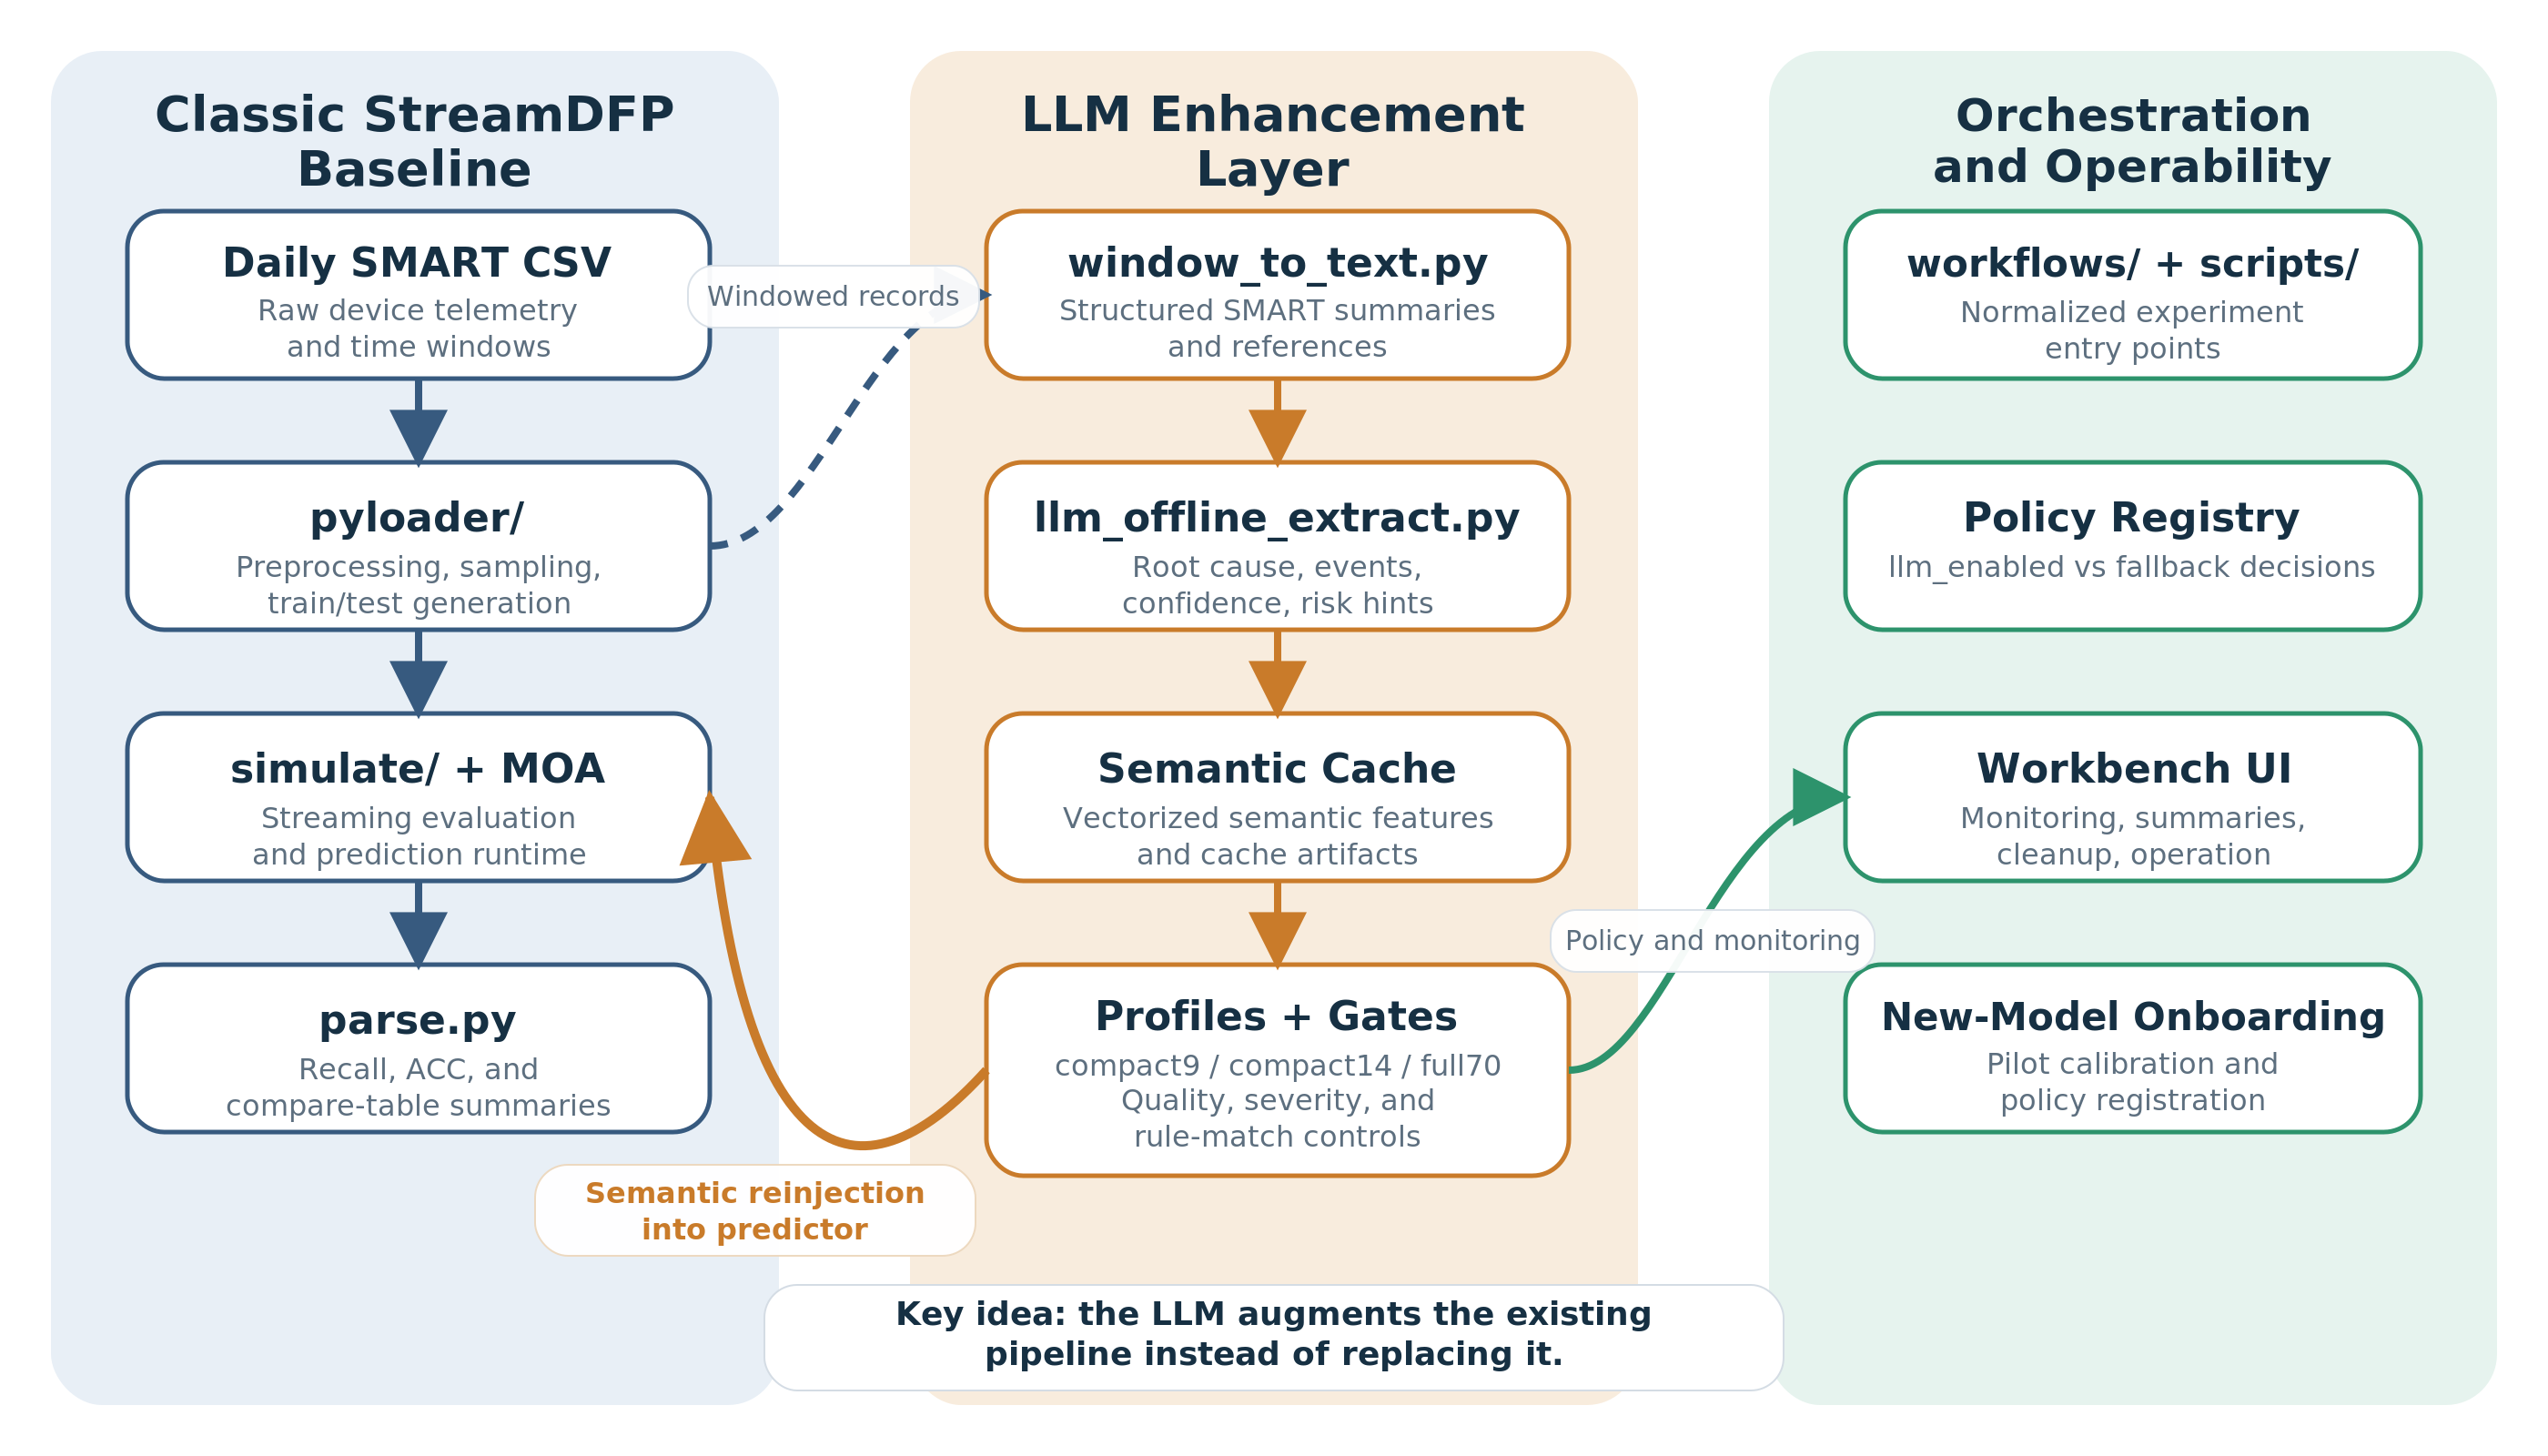
\includegraphics[width=0.84\textwidth,height=\textheight]{frontend_exports/figure1_overall_architecture.png}
\caption{Overall architecture of the StreamDFP-LLM extension.}
\end{figure}

\hypertarget{streamdfp-baseline}{%
\subsection{3.2 StreamDFP Baseline}\label{streamdfp-baseline}}

The baseline remains the reference execution path for all comparisons.

\texttt{daily\ SMART\ CSV\ -\textgreater{}\ pyloader/run.py\ -\textgreater{}\ simulate.Simulate\ +\ MOA\ -\textgreater{}\ parse.py}

\texttt{pyloader/run.py} is the main Python-side entry point. It reads
the raw SMART data, constructs time-windowed samples, and writes the
train/test directories consumed by the Java simulation layer.
Importantly, the current implementation also acts as the reintegration
point for LLM features through logic such as policy loading, gate
application, and cache loading. This means that the baseline and the
LLM-enhanced workflow share the same downstream evaluation path.

The Java layer under \texttt{simulate/} and \texttt{moa/} executes the
final predictive run. Methodologically, this is important because it
prevents a common evaluation error: comparing an LLM-enhanced method and
a baseline under different runtime protocols. In this study, every
claimed gain must be obtained through the same downstream predictor and
the same parser-defined metrics. The stream-learning backbone is
implemented around the MOA framework {[}12{]}.

\hypertarget{llm-enhancement-pipeline}{%
\subsection{3.3 LLM Enhancement
Pipeline}\label{llm-enhancement-pipeline}}

The core methodology is implemented through the \texttt{framework\_v1}
pipeline.

\hypertarget{phase-1-window-summarization}{%
\subsubsection{3.3.1 Phase 1: Window
Summarization}\label{phase-1-window-summarization}}

\texttt{llm/window\_to\_text.py} transforms each SMART time window into
a structured summary rather than a raw numerical dump. The generated
text records the window boundary, data-quality cues, rule-based scores,
top-ranked causes, anomaly evidence, and a final rule prediction. This
design makes the input auditable to humans while remaining sufficiently
constrained for machine extraction.

Phase 1 is also where sampling quality becomes critical. The later mc1
diagnosis showed that an incorrect sequential sampling strategy can
severely degrade downstream extraction quality. Phase 1 should therefore
be regarded not merely as a formatting step, but as part of the
experimental-validity chain.

\hypertarget{phase-2-semantic-extraction}{%
\subsubsection{3.3.2 Phase 2: Semantic
Extraction}\label{phase-2-semantic-extraction}}

\texttt{llm/llm\_offline\_extract.py} sends the structured summary to a
selected backend and extracts a normalized semantic description,
including the inferred root cause, event evidence, risk indication,
hardness estimate, and confidence level. The project supports three
backend families: local Transformers backends, local vLLM backends, and
OpenAI-compatible API backends.

The extracted results are then normalized into cache records containing
semantic attributes, vectorized LLM signals, quality scores, and
rule-matching indicators. This stage constitutes the main bridge between
the language model and the conventional predictive system.

\hypertarget{phase-3-gating-and-reinjection}{%
\subsubsection{3.3.3 Phase 3: Gating and
Reinjection}\label{phase-3-gating-and-reinjection}}

\texttt{llm/scripts/build\_cache\_variant.py} and the Phase 3 grid
scripts evaluate which parts of the cache should actually be injected
back into the predictor. The project commonly uses the compact9,
compact14, and full70 feature profiles, combined with gate settings such
as quality thresholds, severity thresholds, and rule-match constraints.

This phase operationalizes the principle of selective enhancement. Not
every LLM output is trusted, and not every disk model benefits from the
same configuration. Accordingly, the system compares profile variants
under the same baseline protocol and records whether a disk model should
remain on the baseline or be promoted to LLM-enabled operation.

\begin{figure}
\centering
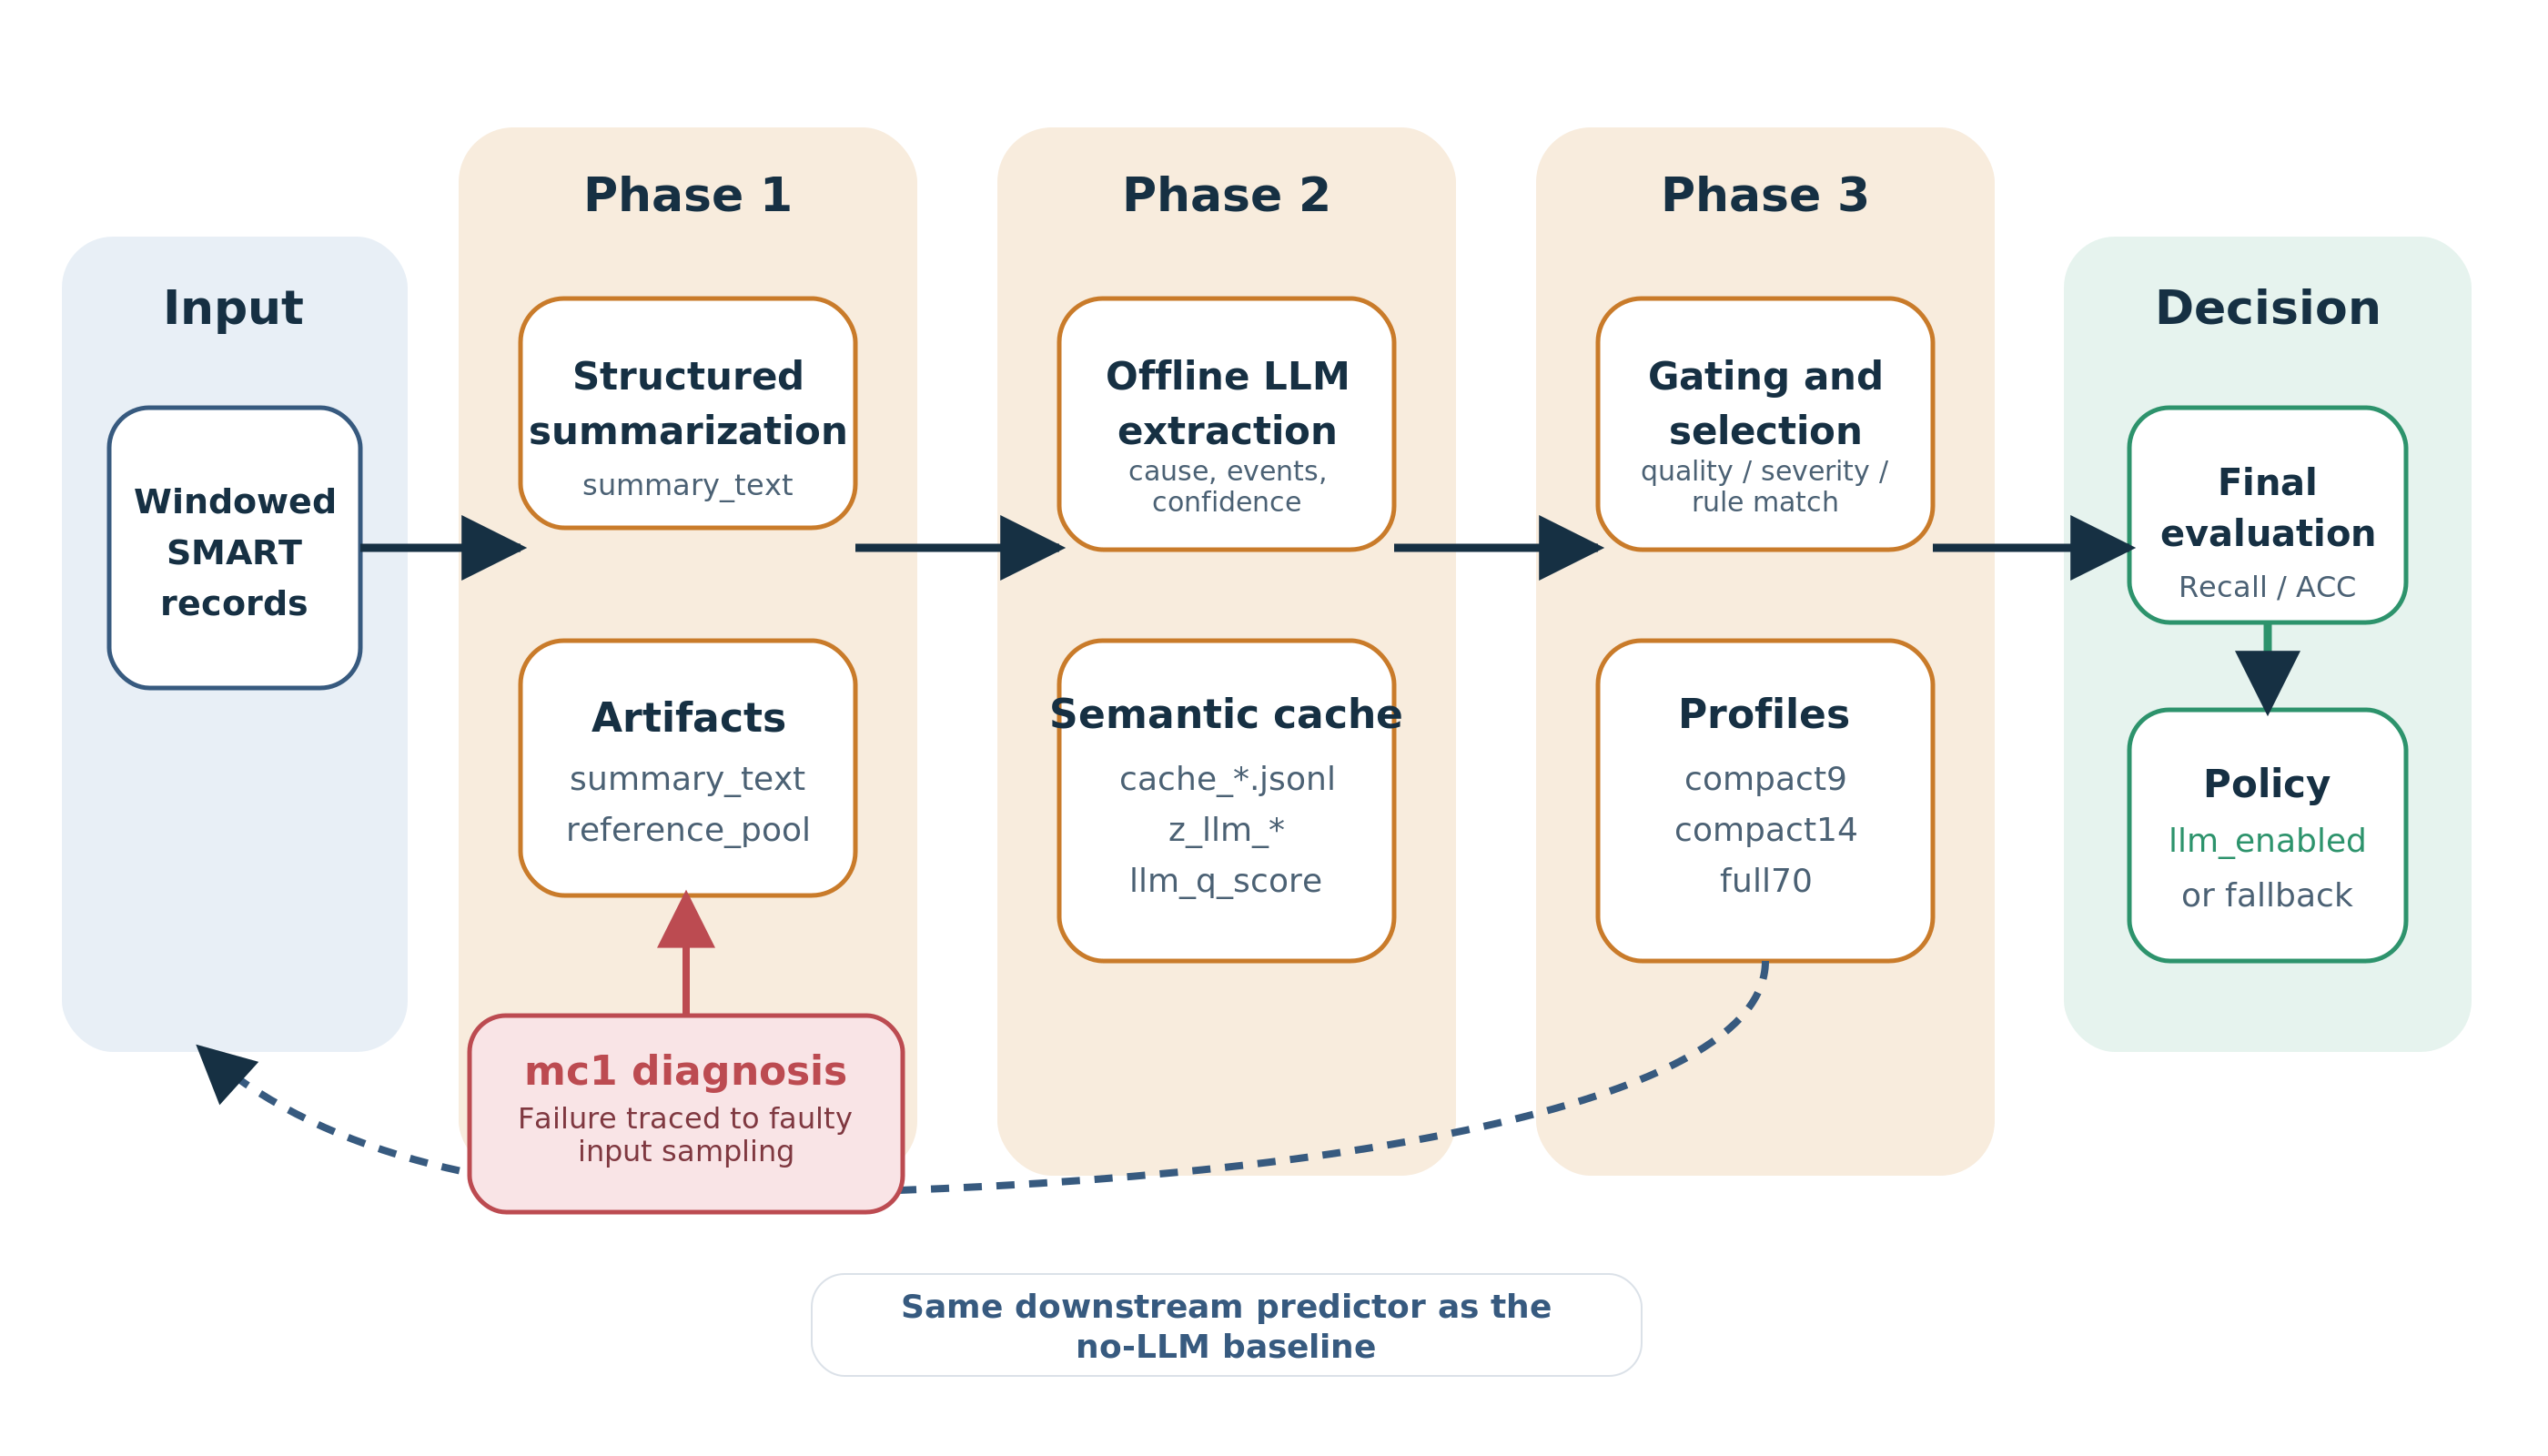
\includegraphics[width=0.82\textwidth,height=\textheight]{frontend_exports/figure2_phase123_pipeline.png}
\caption{Dataflow of the Phase 1-Phase 2-Phase 3 pipeline.}
\end{figure}

\hypertarget{intermediate-artifacts}{%
\subsection{3.4 Intermediate Artifacts}\label{intermediate-artifacts}}

A key design choice is that each stage produces explicit intermediate
artifacts rather than hiding the entire process inside a single
end-to-end script.

Table 2. Phase contract and intermediate artifacts.

\begin{longtable}[]{@{}lllll@{}}
\toprule
\begin{minipage}[b]{0.17\columnwidth}\raggedright
Stage\strut
\end{minipage} & \begin{minipage}[b]{0.17\columnwidth}\raggedright
Main input\strut
\end{minipage} & \begin{minipage}[b]{0.17\columnwidth}\raggedright
Main output\strut
\end{minipage} & \begin{minipage}[b]{0.17\columnwidth}\raggedright
Typical artifact\strut
\end{minipage} & \begin{minipage}[b]{0.17\columnwidth}\raggedright
Why it matters\strut
\end{minipage}\tabularnewline
\midrule
\endhead
\begin{minipage}[t]{0.17\columnwidth}\raggedright
Classic preprocessing\strut
\end{minipage} & \begin{minipage}[t]{0.17\columnwidth}\raggedright
raw daily SMART CSV\strut
\end{minipage} & \begin{minipage}[t]{0.17\columnwidth}\raggedright
train/test-ready windows\strut
\end{minipage} & \begin{minipage}[t]{0.17\columnwidth}\raggedright
generated train/test dirs\strut
\end{minipage} & \begin{minipage}[t]{0.17\columnwidth}\raggedright
establishes the no-LLM baseline input\strut
\end{minipage}\tabularnewline
\begin{minipage}[t]{0.17\columnwidth}\raggedright
Phase 1\strut
\end{minipage} & \begin{minipage}[t]{0.17\columnwidth}\raggedright
windowed SMART records\strut
\end{minipage} & \begin{minipage}[t]{0.17\columnwidth}\raggedright
structured summaries and references\strut
\end{minipage} & \begin{minipage}[t]{0.17\columnwidth}\raggedright
summary text, reference pool\strut
\end{minipage} & \begin{minipage}[t]{0.17\columnwidth}\raggedright
makes each numerical window auditable and LLM-readable\strut
\end{minipage}\tabularnewline
\begin{minipage}[t]{0.17\columnwidth}\raggedright
Phase 2\strut
\end{minipage} & \begin{minipage}[t]{0.17\columnwidth}\raggedright
summary text\strut
\end{minipage} & \begin{minipage}[t]{0.17\columnwidth}\raggedright
structured extraction cache\strut
\end{minipage} & \begin{minipage}[t]{0.17\columnwidth}\raggedright
cache JSONL files\strut
\end{minipage} & \begin{minipage}[t]{0.17\columnwidth}\raggedright
separates LLM inference from downstream evaluation\strut
\end{minipage}\tabularnewline
\begin{minipage}[t]{0.17\columnwidth}\raggedright
Phase 3\strut
\end{minipage} & \begin{minipage}[t]{0.17\columnwidth}\raggedright
Phase 2 cache\strut
\end{minipage} & \begin{minipage}[t]{0.17\columnwidth}\raggedright
gated and compacted variants\strut
\end{minipage} & \begin{minipage}[t]{0.17\columnwidth}\raggedright
phase3 variant JSON\strut
\end{minipage} & \begin{minipage}[t]{0.17\columnwidth}\raggedright
supports profile and gate ablation\strut
\end{minipage}\tabularnewline
\begin{minipage}[t]{0.17\columnwidth}\raggedright
Final evaluation\strut
\end{minipage} & \begin{minipage}[t]{0.17\columnwidth}\raggedright
chosen variant + original predictor\strut
\end{minipage} & \begin{minipage}[t]{0.17\columnwidth}\raggedright
metric CSV and summaries\strut
\end{minipage} & \begin{minipage}[t]{0.17\columnwidth}\raggedright
parsed metrics CSV\strut
\end{minipage} & \begin{minipage}[t]{0.17\columnwidth}\raggedright
determines whether LLM should be enabled\strut
\end{minipage}\tabularnewline
\bottomrule
\end{longtable}

This explicit phase contract is important not only for engineering
convenience but also for research validity. It makes it possible to
localize where an error first appears. The mc1 case provides the
clearest example: the observed failure was traced back to Phase 1 input
sampling rather than to the final predictor alone.

\hypertarget{acceptance-criteria-and-policy}{%
\subsection{3.5 Acceptance Criteria and
Policy}\label{acceptance-criteria-and-policy}}

The main acceptance rule used in the retained public summaries is as
follows.

\begin{itemize}
\tightlist
\item
  \texttt{Recall(LLM)\ \textgreater{}=\ Recall(noLLM)}
\item
  \texttt{ACC(LLM)\ \textgreater{}=\ ACC(noLLM)\ -\ 1.0pp}
\end{itemize}

This rule reflects the fact that missing failure cases is more costly
than a small fluctuation in overall accuracy. It also prevents the
report from overstating modest gains obtained at the expense of failure
recall. Under this rule, the final output is not a single global
configuration but a disk-model-level policy table indicating where LLM
enhancement is acceptable.

\hypertarget{onboarding-and-reproducibility}{%
\subsection{3.6 Onboarding and
Reproducibility}\label{onboarding-and-reproducibility}}

The system also defines an onboarding path for new disk models:

new model -\textgreater{} no-LLM baseline -\textgreater{} pilot20k Phase
1/Phase 2/Phase 3 -\textgreater{} guard check -\textgreater{} policy
registration

\begin{figure}
\centering
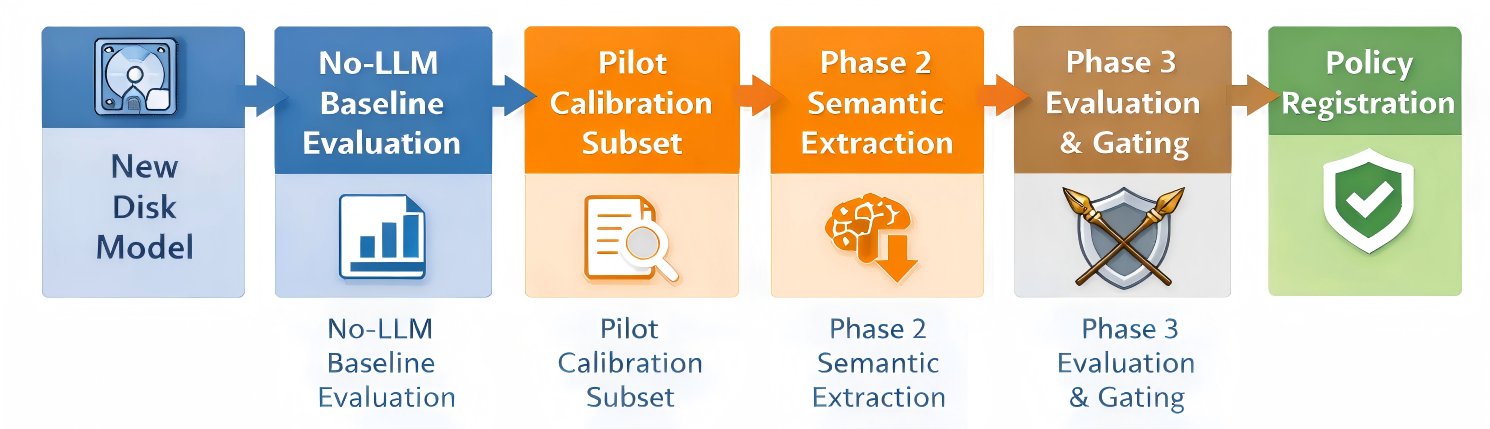
\includegraphics[width=0.72\textwidth,height=\textheight]{../write_report/New-Model Onboarding Workflow.png}
\caption{New-model onboarding workflow used in the current calibration
and policy-registration branch.}
\end{figure}

This branch is methodologically important because it turns the project
from a collection of one-off experiments into a repeatable research
workflow. The same design logic is reflected in the operability layer:

\begin{itemize}
\tightlist
\item
  \texttt{scripts/} keeps historically faithful experiment entry points
\item
  \texttt{workflows/} provides normalized wrapper names
\item
  \texttt{ui/server.py} and \texttt{run\_workbench.sh} expose a
  lightweight local workbench
\end{itemize}

The implementation associated with this report is maintained in the
GitHub repository StreamDFP-LLM-Extension:
https://github.com/zmdlmd/StreamDFP-LLM-Extension. The repository
records the current hybrid extension branch, workflow wrappers,
figure-generation assets, and retained experiment artifacts used in this
report.

The workbench is not merely a launcher. It also summarizes results,
monitors jobs, and manages experiment artifacts. For a research system
that combines Python, Java, local LLM inference, API inference, and many
cached artifacts, this layer should be regarded as part of the
methodology rather than as a cosmetic add-on. A representative interface
snapshot is provided in the Appendix.

\hypertarget{experiments-and-results}{%
\section{4. Experiments and Results}\label{experiments-and-results}}

\hypertarget{data-and-evaluation-setting}{%
\subsection{4.1 Data and Evaluation
Setting}\label{data-and-evaluation-setting}}

The repository does not ship the raw datasets, but the documented public
reproduction path expects HDD data under \texttt{data/data\_2014/2014/}
in a Backblaze-style daily SMART format {[}13{]}. For the HDD branch,
the retained \texttt{framework\_v1} metric contract uses the evaluation
window \texttt{2014-09-01\ \textasciitilde{}\ 2014-11-09}. The merged
public summaries cover 12 HDD disk models. These HDD results form the
main basis for the current policy discussion.

The SSD-side case reported in this report is mc1, which is treated
separately from the HDD models. Its repaired calibration branch uses the
pilot20k\_stratified\_v2 input and covers the interval 2018-02-01 to
2018-03-13 in window\_end\_time. The repository consistently treats mc1
as an SSD pilot case rather than as a directly comparable member of the
HDD set. HDD and mc1 should therefore be discussed within the same
report, but they should not be merged into a single absolute
cross-medium ranking. The SSD branch is consistent with the public
Alibaba SSD line of work and dataset release described in Xu et
al.~{[}14{]}.

The role of pilot20k is also important. It is not merely a small-sample
shortcut; rather, it serves as an admission-test branch for model
calibration and new-disk-model onboarding before a policy decision is
registered.

\hypertarget{evaluation-protocol}{%
\subsection{4.2 Evaluation Protocol}\label{evaluation-protocol}}

All claims in this report follow a single methodological requirement:
the LLM-enhanced system must be compared against the no-LLM baseline
under the same downstream prediction chain and the same metric parser.
The principal metrics used in the repository are Recall\_c1 and ACC.

The acceptance rule described in Section 3.5 is used to decide whether a
disk model is allowed to adopt LLM enhancement. This is a conservative
protocol that prioritizes failure recall over small changes in overall
accuracy.

In the retained public summaries, the merged report over all tracked
models records PASS = 9, FALLBACK = 4, and N/A = 0 across 13 tracked
entries, where one of the PASS entries is the separate SSD case
mc1\_pilot20k. This leaves 8 accepted HDD models and 4 fallback HDD
models in the present policy picture.

\hypertarget{hdd-policy-snapshot}{%
\subsection{4.3 HDD Policy Snapshot}\label{hdd-policy-snapshot}}

Table 3. HDD model policy snapshot under the locked local baseline.

\begin{longtable}[]{@{}ll@{}}
\toprule
\begin{minipage}[b]{0.47\columnwidth}\raggedright
Status\strut
\end{minipage} & \begin{minipage}[b]{0.47\columnwidth}\raggedright
HDD models\strut
\end{minipage}\tabularnewline
\midrule
\endhead
\begin{minipage}[t]{0.47\columnwidth}\raggedright
enabled\strut
\end{minipage} & \begin{minipage}[t]{0.47\columnwidth}\raggedright
hds723030ala640, hgsthms5c4040ale640, hi7, hitachihds5c4040ale630,
st3000dm001, st31500341as, st31500541as, wdcwd30efrx\strut
\end{minipage}\tabularnewline
\begin{minipage}[t]{0.47\columnwidth}\raggedright
fallback\strut
\end{minipage} & \begin{minipage}[t]{0.47\columnwidth}\raggedright
hds5c3030ala630, hms5c4040ble640, st4000dm000, wdcwd10eads\strut
\end{minipage}\tabularnewline
\bottomrule
\end{longtable}

This split shows that the central claim of the project is not simply
that LLM enhancement is superior to the no-LLM baseline on HDD in
general. The claim is narrower and therefore more defensible: under a
fixed acceptance rule, some disk models exhibit sufficient evidence to
justify semantic enhancement, whereas others should remain on the
original baseline.

\hypertarget{hdd-model-comparison}{%
\subsection{4.4 HDD Model Comparison}\label{hdd-model-comparison}}

Table 4 compares three candidate models: Qwen3-4B-Instruct-2507,
Qwen3.5-4B, and Qwen3.5-Plus.

Table 4. HDD cross-model comparison under the retained evaluation
protocol.

\begin{longtable}[]{@{}lrr@{}}
\toprule
Model & Enabled HDD models & Avg. Delta Recall\tabularnewline
\midrule
\endhead
Qwen3-Instruct & 8 & 18.0903\tabularnewline
Qwen3.5-4B & 7 & 19.2081\tabularnewline
Qwen3.5-Plus & 7 & 20.1520\tabularnewline
\bottomrule
\end{longtable}

\begin{figure}
\centering
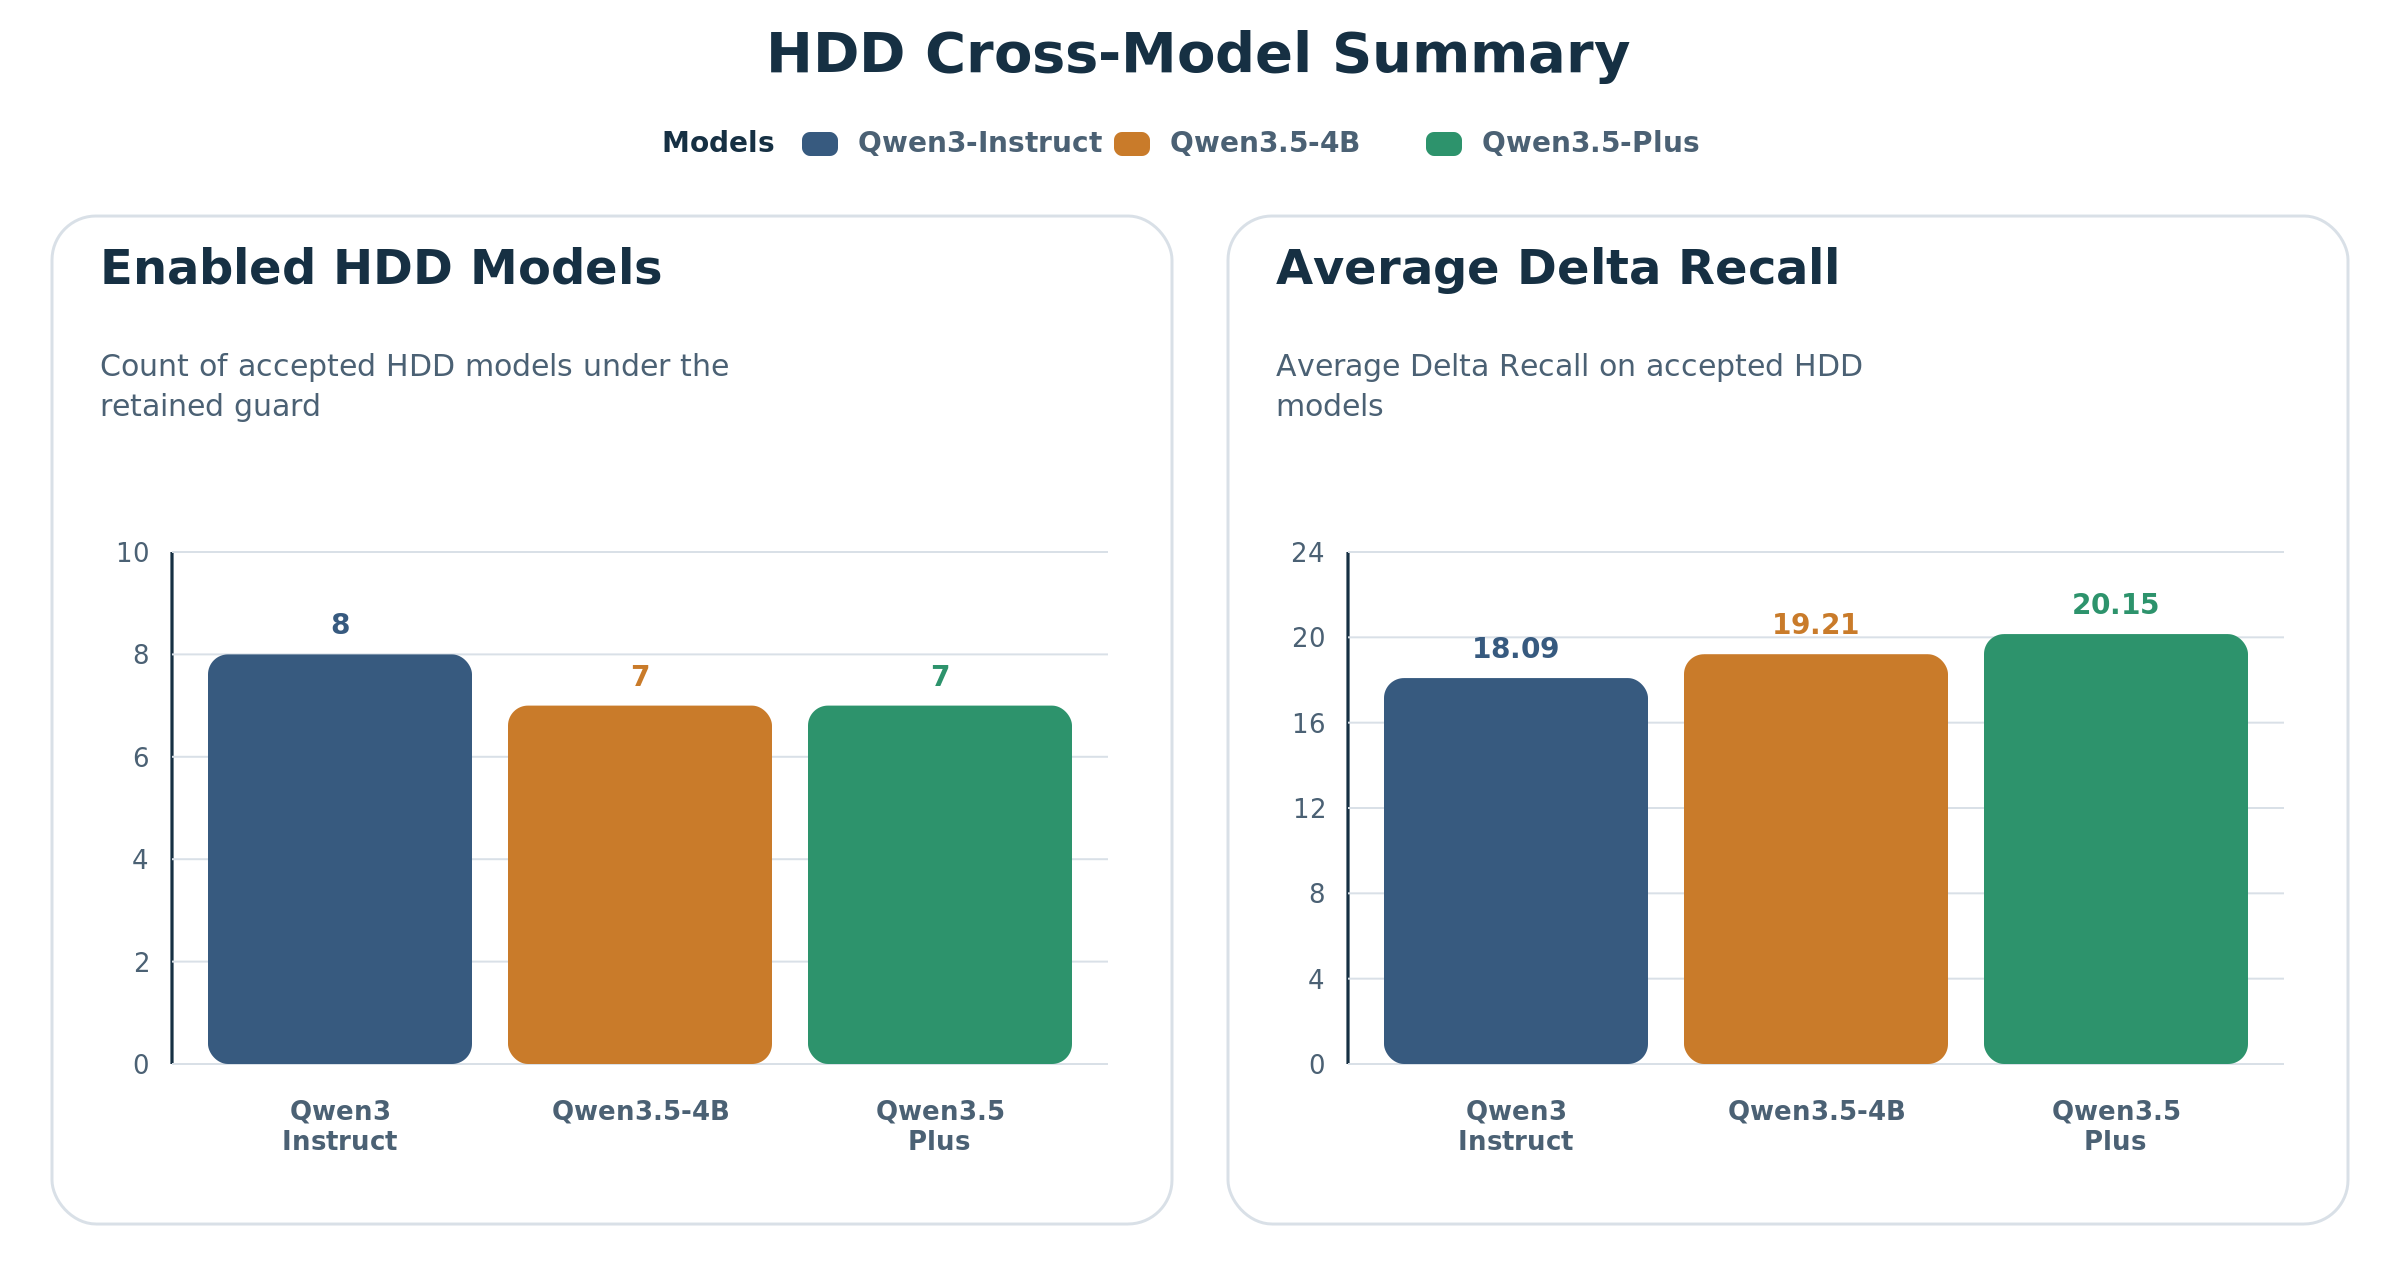
\includegraphics[width=0.84\textwidth,height=\textheight]{frontend_exports/figure3_hdd_cross_model_summary.png}
\caption{HDD cross-model comparison under the retained
evaluation protocol.}
\end{figure}

Three observations emerge. First, the preferred model depends on the
optimization target. Qwen3-4B-Instruct-2507 enables the largest number
of HDD models and is therefore attractive when broader coverage is the
priority. Second, Qwen3.5-Plus yields the highest average Delta Recall
over accepted models, but does not increase the number of enabled
models. Third, Qwen3.5-4B occupies an intermediate numerical position
while offering a less favorable runtime profile in the current
implementation. More importantly, the retained policy records show that
different models prefer different profile-gate combinations, including
compact9, compact14, and full70. The observed benefit therefore does not
arise from adding a generic semantic block; rather, it arises from
controlled semantic compaction combined with selective gating.

\begin{figure}
\centering
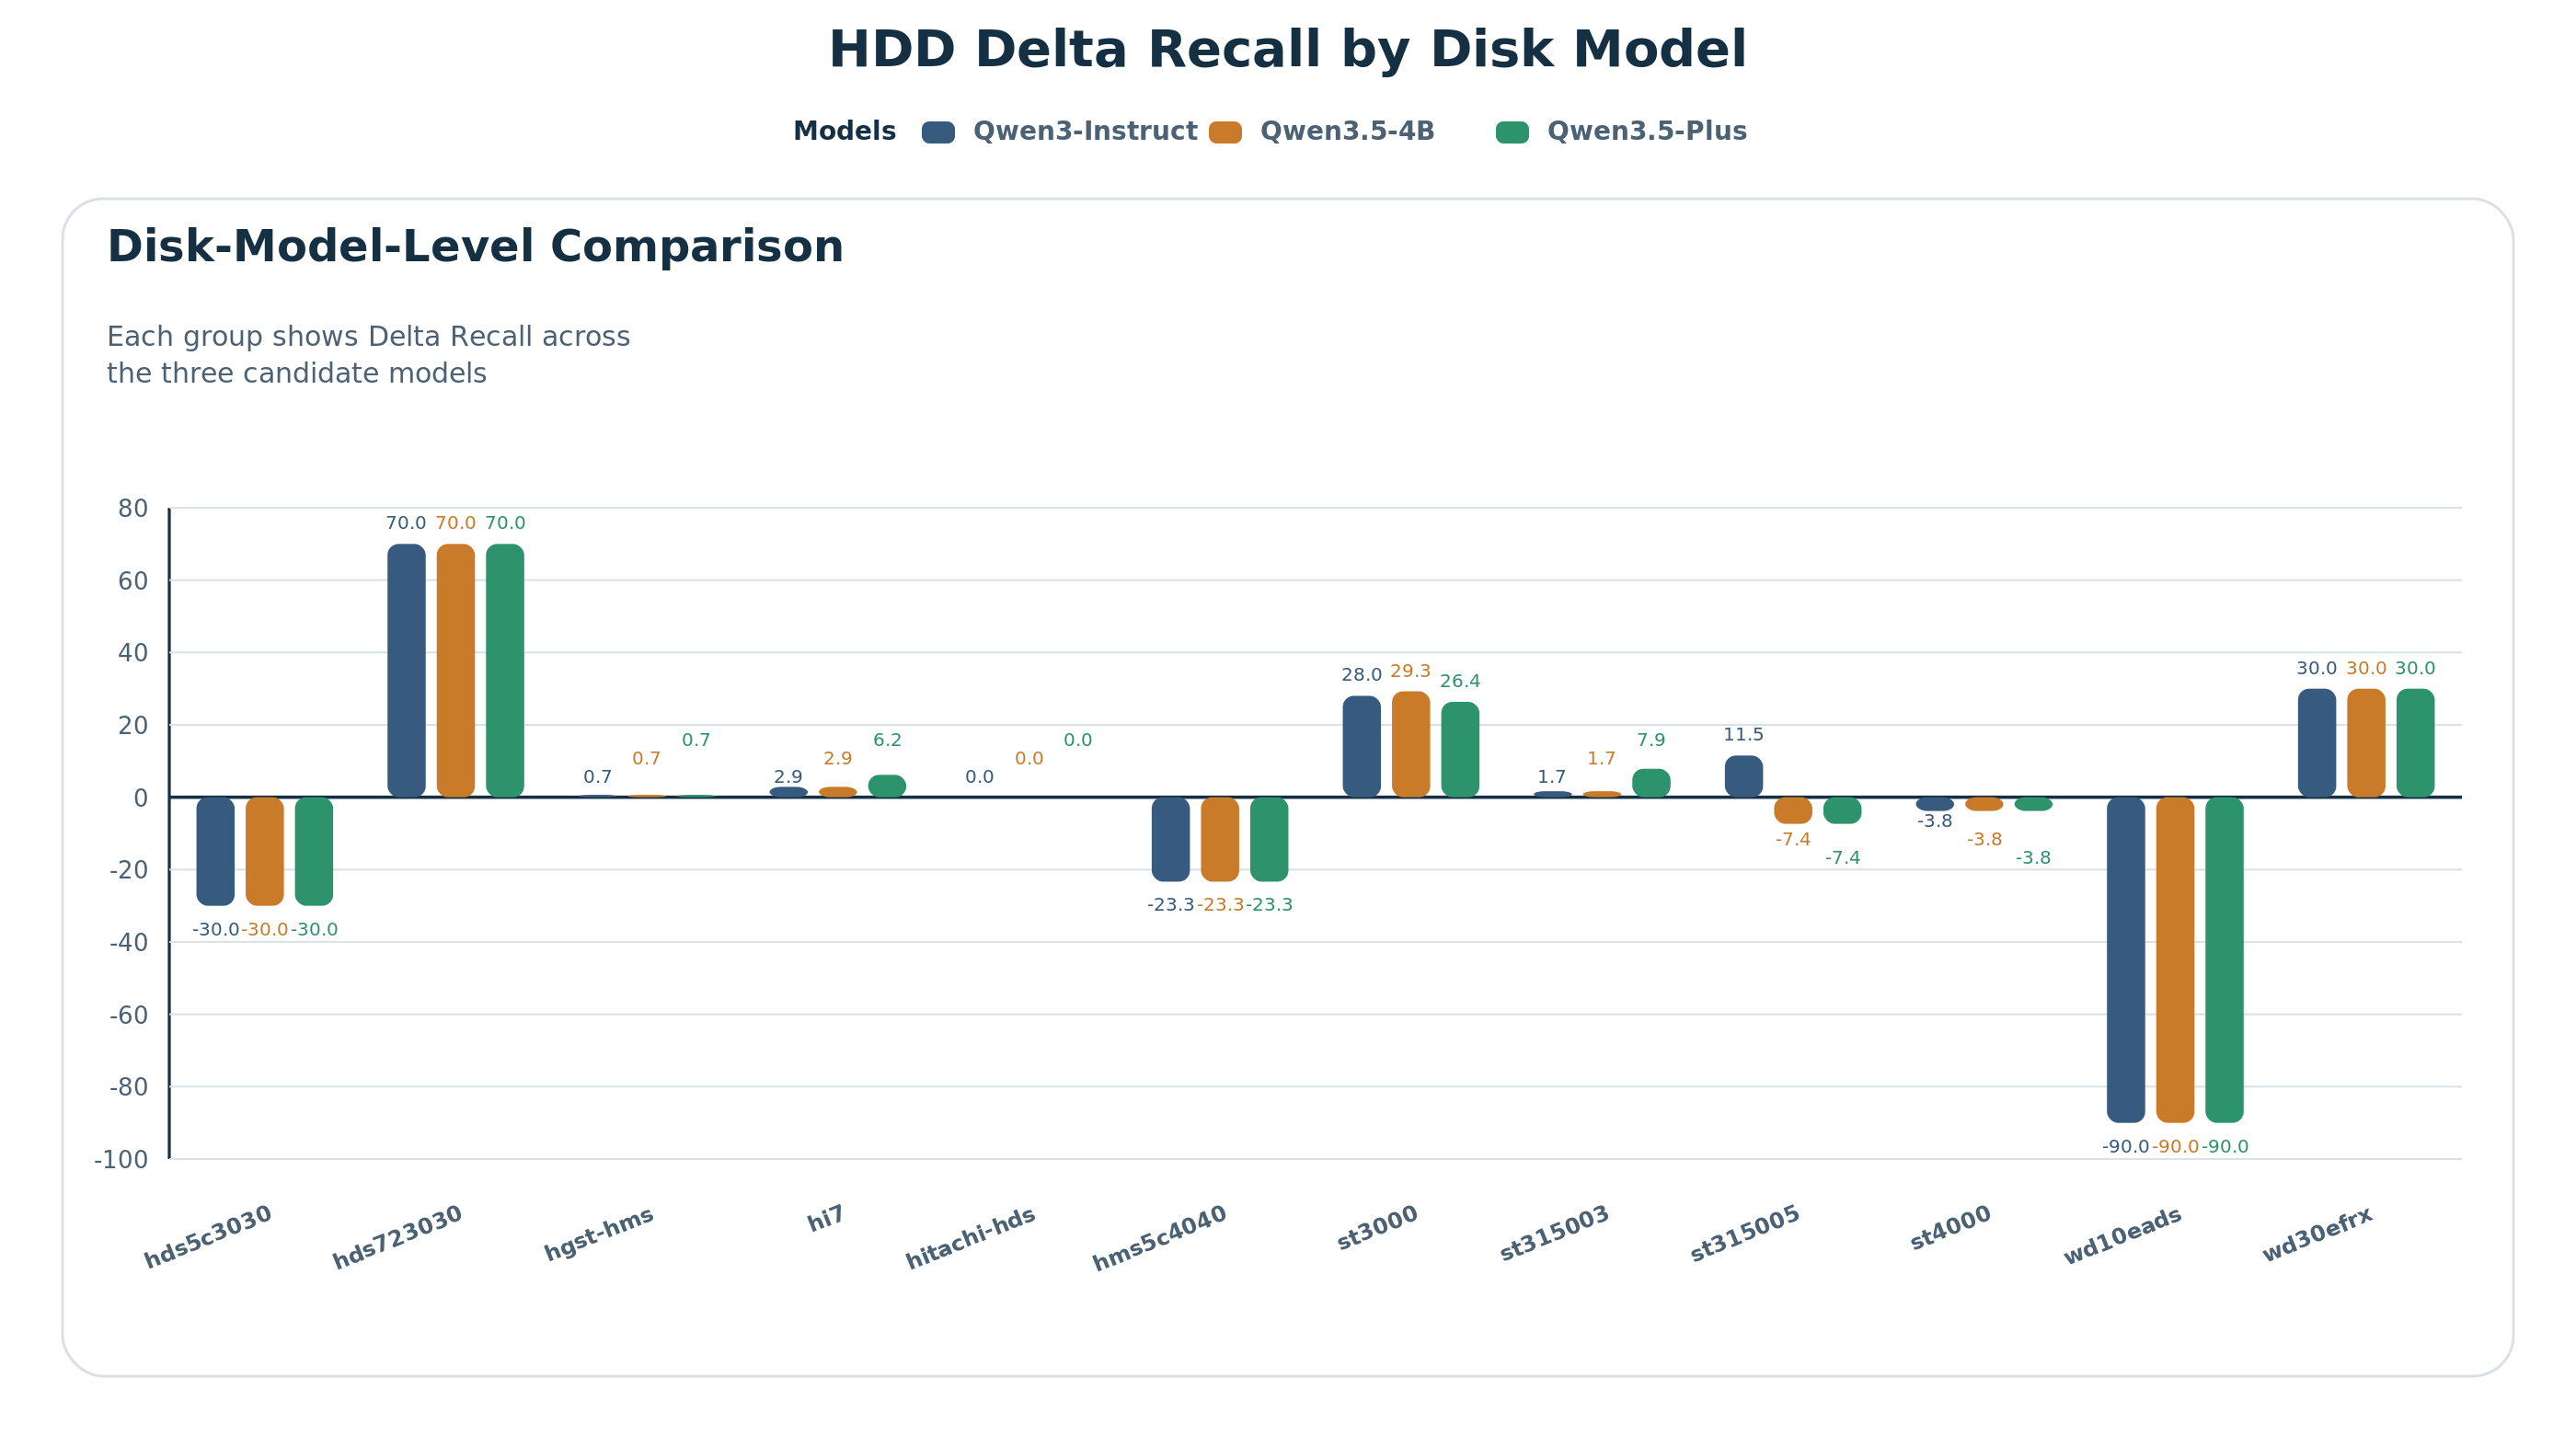
\includegraphics[width=0.84\textwidth,height=\textheight]{frontend_exports/figure4_hdd_delta_by_disk_model.png}
\caption{HDD Delta Recall by disk model across the three
candidate models.}
\end{figure}

\hypertarget{the-mc1-case-study}{%
\subsection{4.5 The mc1 Case Study}\label{the-mc1-case-study}}

The mc1 SSD case is methodologically important because it initially
appeared to indicate a failure of the LLM-enhanced pipeline. Subsequent
diagnosis showed that the dominant issue did not originate in the model
family itself, but in the input data chain. The earlier mc1 experiment
used a faulty sequential sampling strategy that concentrated many
samples in the earliest days and produced poor contextual coverage for a
30-day window. The consequence was a high rate of unknown outputs,
sparse active features, and degenerate Phase 3 behavior.

The repaired version, pilot20k\_stratified\_v2, rebuilt the input with a
stratified\_day\_disk sampling strategy over a broader time range and
reconstructed the reference pool accordingly. This correction
substantially improved the validity of the experiment.

\begin{figure}
\centering
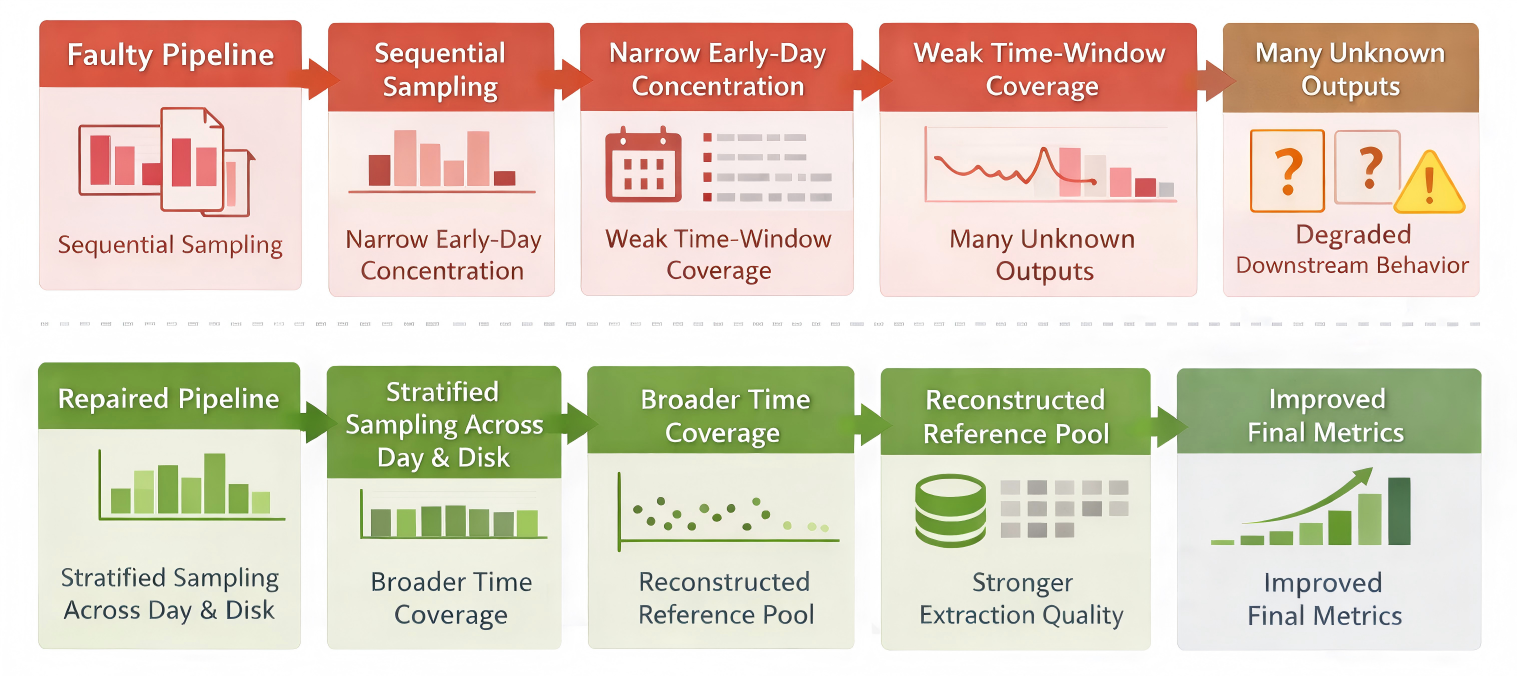
\includegraphics[width=0.72\textwidth,height=\textheight]{../write_report/mc1 Failure-and-Repair Storyline.png}
\caption{Failure diagnosis and repair path for the mc1 evaluation
pipeline.}
\end{figure}

The principal result is that the best retained Phase 3 configuration is
identical for all three compared models:

Table 5. Best retained Phase 3 outcome on repaired mc1.

\begin{longtable}[]{@{}llrrrr@{}}
\toprule
Case & Best profile & Recall & ACC & Delta Recall & Delta
ACC\tabularnewline
\midrule
\endhead
Baseline & - & 97.7704 & 99.4956 & 0.0000 & 0.0000\tabularnewline
Repaired mc1 + LLM & compact14, q0/s0/r0 & 100.0000 & 99.5489 & +2.2296
& +0.0532\tabularnewline
\bottomrule
\end{longtable}

This case study is methodologically significant for two reasons. First,
it shows that a defective data pipeline can masquerade as a model
failure. Second, it shows that, once the input pipeline is repaired, the
task itself is not inherently unsuitable for LLM augmentation.

\hypertarget{phase-2-quality-on-repaired-mc1}{%
\subsection{4.6 Phase 2 Quality on Repaired
mc1}\label{phase-2-quality-on-repaired-mc1}}

Although the three models converge to the same best Phase 3 result on
repaired mc1, their Phase 2 extraction quality differs substantially.

Table 6. Phase 2 extraction-quality comparison on repaired mc1.

\begin{longtable}[]{@{}lrrrrrr@{}}
\toprule
\begin{minipage}[b]{0.09\columnwidth}\raggedright
Model\strut
\end{minipage} & \begin{minipage}[b]{0.12\columnwidth}\raggedleft
Unknown \%\strut
\end{minipage} & \begin{minipage}[b]{0.12\columnwidth}\raggedleft
Non-unknown \%\strut
\end{minipage} & \begin{minipage}[b]{0.12\columnwidth}\raggedleft
Mapped event \%\strut
\end{minipage} & \begin{minipage}[b]{0.12\columnwidth}\raggedleft
Avg. confidence\strut
\end{minipage} & \begin{minipage}[b]{0.12\columnwidth}\raggedleft
Avg. risk hint\strut
\end{minipage} & \begin{minipage}[b]{0.12\columnwidth}\raggedleft
Avg. q-score\strut
\end{minipage}\tabularnewline
\midrule
\endhead
\begin{minipage}[t]{0.09\columnwidth}\raggedright
Qwen3.5 4B\strut
\end{minipage} & \begin{minipage}[t]{0.12\columnwidth}\raggedleft
92.4450\%\strut
\end{minipage} & \begin{minipage}[t]{0.12\columnwidth}\raggedleft
7.5550\%\strut
\end{minipage} & \begin{minipage}[t]{0.12\columnwidth}\raggedleft
77.4600\%\strut
\end{minipage} & \begin{minipage}[t]{0.12\columnwidth}\raggedleft
0.2247\strut
\end{minipage} & \begin{minipage}[t]{0.12\columnwidth}\raggedleft
0.2105\strut
\end{minipage} & \begin{minipage}[t]{0.12\columnwidth}\raggedleft
0.2470\strut
\end{minipage}\tabularnewline
\begin{minipage}[t]{0.09\columnwidth}\raggedright
Qwen3.5 Plus\strut
\end{minipage} & \begin{minipage}[t]{0.12\columnwidth}\raggedleft
92.3250\%\strut
\end{minipage} & \begin{minipage}[t]{0.12\columnwidth}\raggedleft
7.6750\%\strut
\end{minipage} & \begin{minipage}[t]{0.12\columnwidth}\raggedleft
90.1950\%\strut
\end{minipage} & \begin{minipage}[t]{0.12\columnwidth}\raggedleft
0.3727\strut
\end{minipage} & \begin{minipage}[t]{0.12\columnwidth}\raggedleft
0.2779\strut
\end{minipage} & \begin{minipage}[t]{0.12\columnwidth}\raggedleft
0.2974\strut
\end{minipage}\tabularnewline
\begin{minipage}[t]{0.09\columnwidth}\raggedright
Qwen3 Instruct\strut
\end{minipage} & \begin{minipage}[t]{0.12\columnwidth}\raggedleft
91.5550\%\strut
\end{minipage} & \begin{minipage}[t]{0.12\columnwidth}\raggedleft
8.4450\%\strut
\end{minipage} & \begin{minipage}[t]{0.12\columnwidth}\raggedleft
90.7750\%\strut
\end{minipage} & \begin{minipage}[t]{0.12\columnwidth}\raggedleft
0.8547\strut
\end{minipage} & \begin{minipage}[t]{0.12\columnwidth}\raggedleft
0.7133\strut
\end{minipage} & \begin{minipage}[t]{0.12\columnwidth}\raggedleft
0.4503\strut
\end{minipage}\tabularnewline
\bottomrule
\end{longtable}

\begin{figure}
\centering
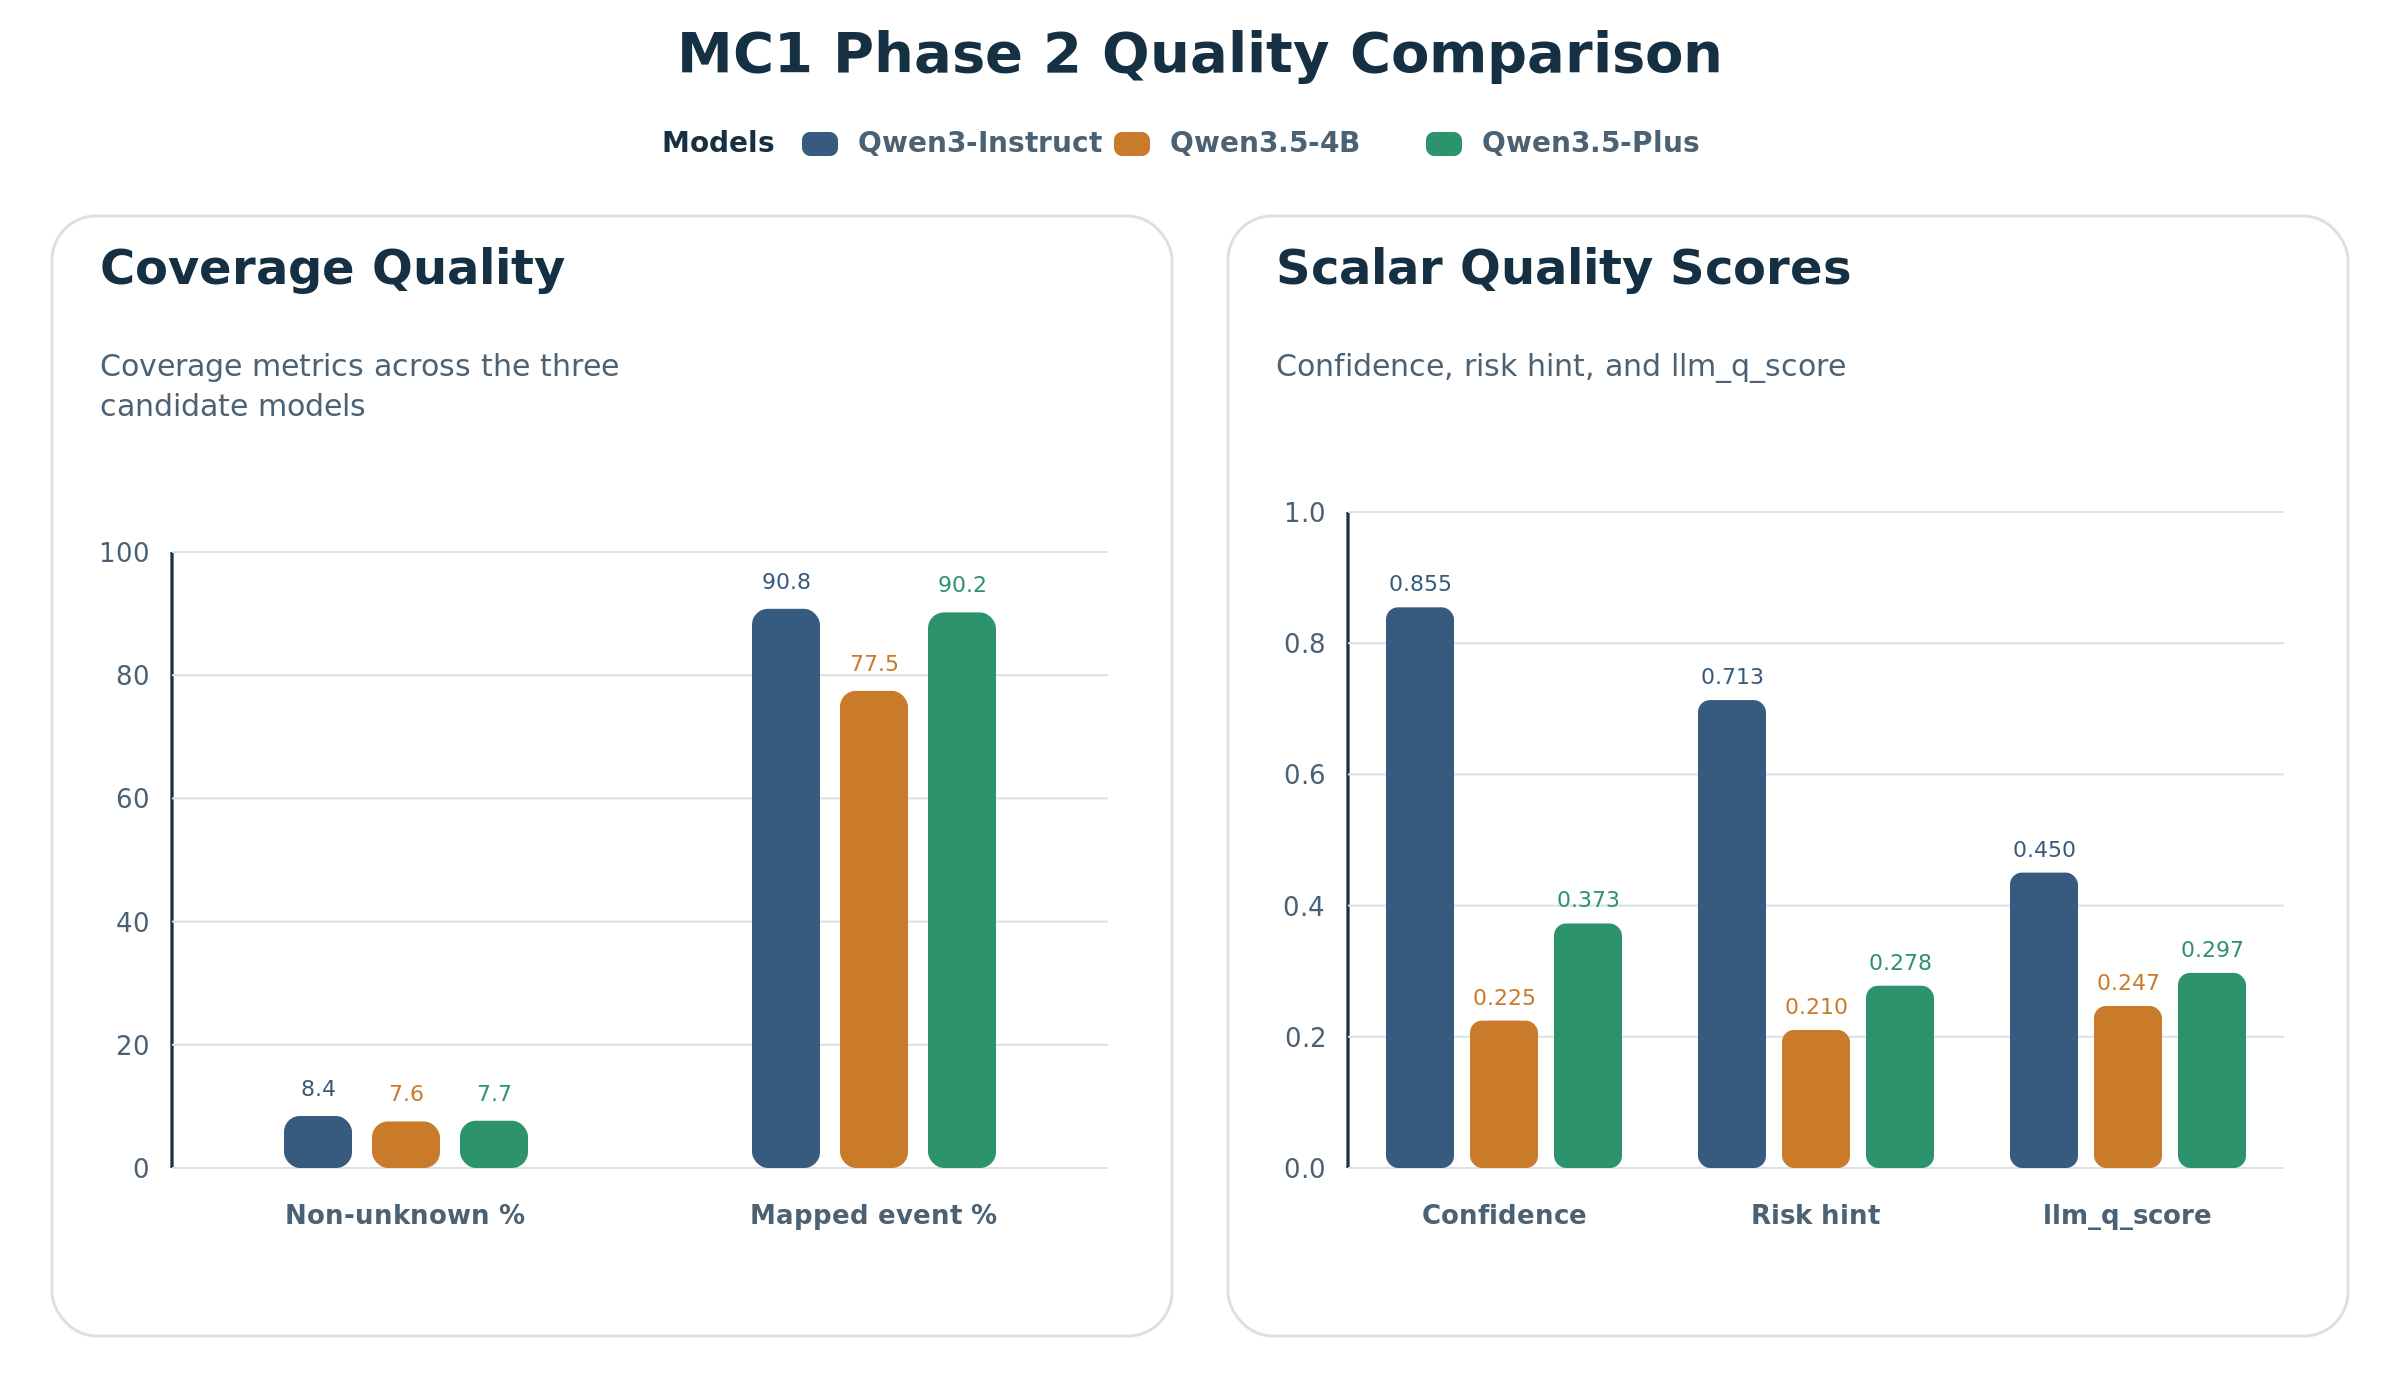
\includegraphics[width=0.84\textwidth,height=\textheight]{frontend_exports/figure5_mc1_phase2_quality.png}
\caption{MC1 Phase2 quality comparison on repaired
stratified\_v2 input.}
\end{figure}

The Phase 2 comparison indicates that Qwen3-4B-Instruct-2507 is the
strongest local default, Qwen3.5-Plus is the most practical API-side
comparison branch, and Qwen3.5-4B matches the best final Phase 3 outcome
only at a higher engineering cost and with weaker extraction quality.
This distinction is important because a report based solely on the best
final Phase 3 metric could incorrectly suggest that the three models are
interchangeable. The Phase 2 statistics show that best-case predictive
performance, extraction quality, and engineering cost are related but
distinct dimensions.

\hypertarget{validity}{%
\subsection{4.7 Validity}\label{validity}}

The present results are sufficient to support the main methodological
claims of a first-term report, but they should still be interpreted with
caution. With respect to internal validity, the project is in a
comparatively strong position because the central comparisons return to
a single metric contract, a single baseline definition, and explicit
intermediate artifacts. The mc1 repair further strengthens internal
validity by showing that an apparently contradictory result can be
explained and corrected through pipeline-level diagnosis. External
validity remains more limited. The present registry is tied to the
current disk-model set, prompt structure, and data ranges. The findings
should therefore be interpreted as evidence that selective LLM
enhancement is feasible and useful under the present protocol, not as
proof that the same policy will necessarily generalize to unseen periods
or substantially different disk families.

\hypertarget{model-recommendation}{%
\subsection{4.8 Model Recommendation}\label{model-recommendation}}

Taken together, the first-term evidence supports a provisional model
recommendation. Qwen3-4B-Instruct-2507 should serve as the default local
base model, Qwen3.5-Plus should be retained as the API-side comparison
branch, and Qwen3.5-4B should not be treated as the primary local option
unless the runtime setup is specifically optimized for it. This
recommendation is not based solely on the best metric value; it also
reflects runtime stability, deployment cost, and reproducibility
considerations.

\begin{figure}
\centering
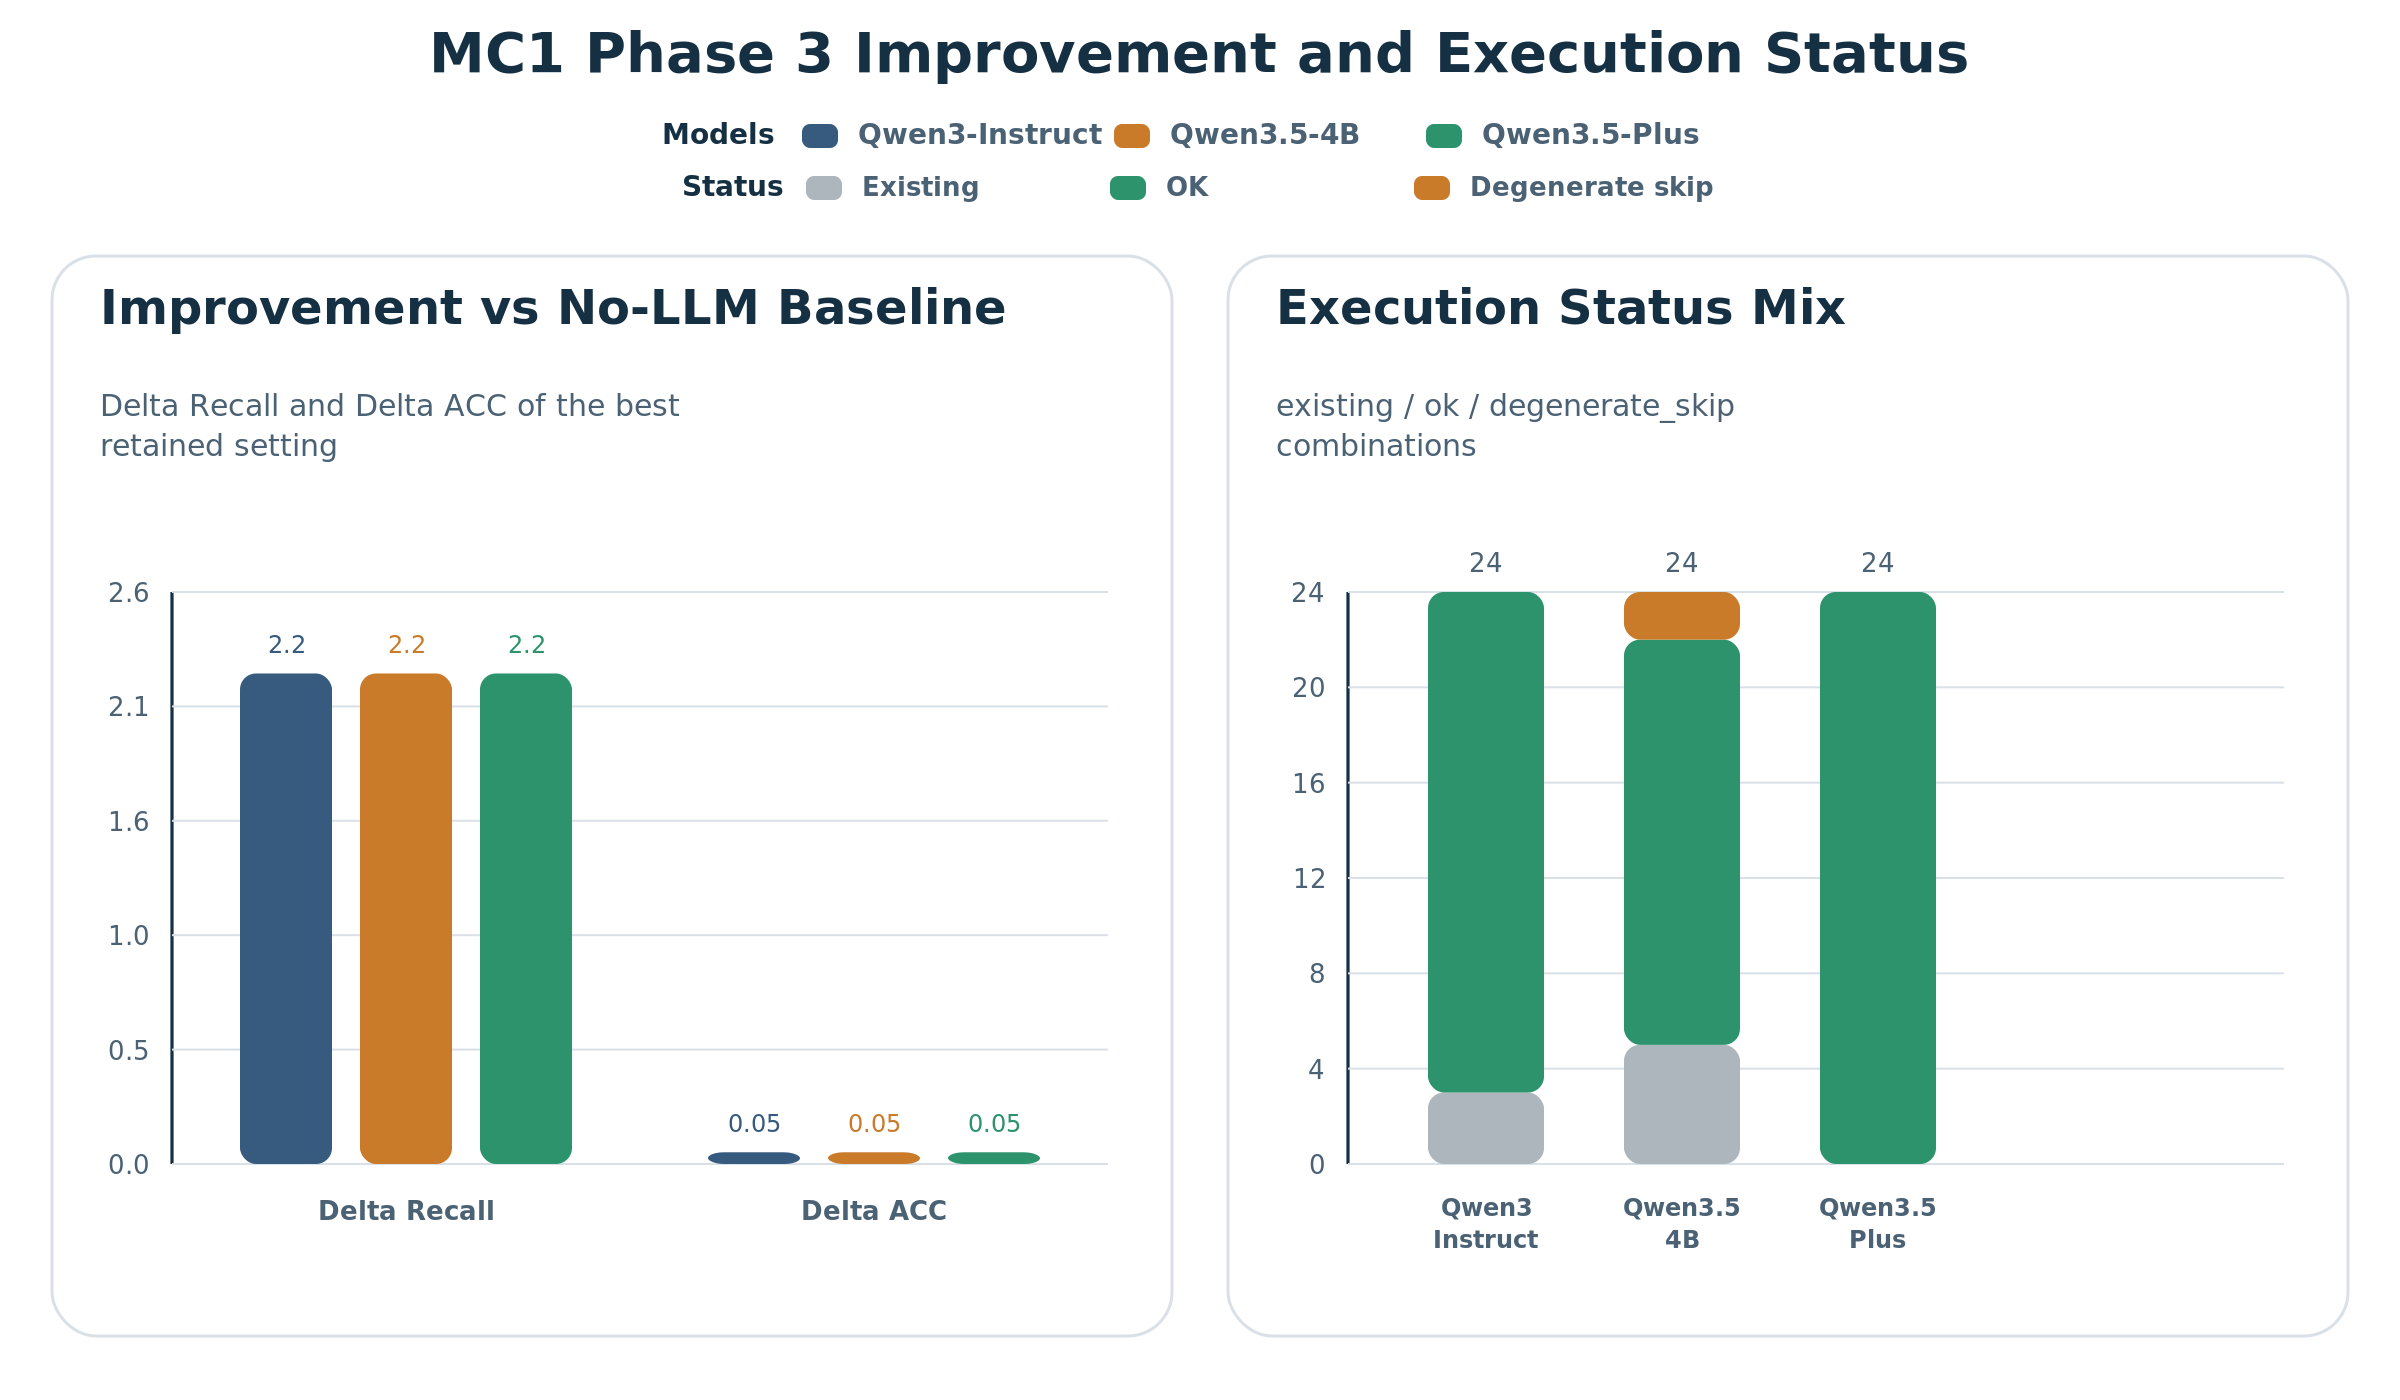
\includegraphics[width=0.84\textwidth,height=\textheight]{frontend_exports/figure6_mc1_phase3_summary.png}
\caption{MC1 Phase3 best result and execution profile across
the three candidate models.}
\end{figure}

\hypertarget{conclusion-and-future-work}{%
\section{5. Conclusion and Future
Work}\label{conclusion-and-future-work}}

\hypertarget{conclusion}{%
\subsection{5.1 Conclusion}\label{conclusion}}

This first-term study shows that extending StreamDFP with structured LLM
signals is both feasible and methodologically meaningful when the
enhancement is evaluated under the same baseline pipeline. The project
establishes a complete three-stage workflow for semantic signal
construction, offline extraction, and gated reinjection. It also shows
that the value of LLM augmentation is selective rather than universal:
some disk models benefit, some should remain on the baseline, and the
final decision should be represented as a policy rather than as a
one-off observation. The mc1 repair case is especially important because
it shows that failure in a hybrid system may originate in the data chain
rather than in the model itself, and that repairing the sampling
pipeline can restore measurable gains under a fixed evaluation rule.

\hypertarget{discussion}{%
\subsection{5.2 Discussion}\label{discussion}}

At the end of the first term, the project is best understood as a
validated research prototype rather than a finished production system.
Its strongest contribution is not a claim of universal performance
superiority; rather, it is the methodological demonstration that
semantic extraction can be integrated into an existing predictive
pipeline without sacrificing comparability, and that policy decisions
can be made conservatively at the disk-model level. Interpreted in this
way, the project contributes a disciplined evaluation loop, a verified
diagnosis of a major failure case, and a reproducible basis for
subsequent calibration and extension.

\hypertarget{limitations}{%
\subsection{5.3 Limitations}\label{limitations}}

The current system still has several limitations.

\begin{enumerate}
\def\labelenumi{\arabic{enumi}.}
\tightlist
\item
  There are still many historical scripts, which increases maintenance
  cost even though reproducibility is preserved.
\item
  Phase 3 remains computationally expensive, especially for cases that
  generate large numbers of train/test artifacts and Java simulation
  outputs.
\item
  Local inference quality and stability still depend on backend-specific
  implementation details.
\item
  The current policy mechanism is still mainly offline and
  disk-model-level, rather than dynamically adaptive online.
\item
  Full reproduction still depends on external resources such as local
  model checkpoints, GPU capacity, API quota, and storage space.
\end{enumerate}

\hypertarget{future-work}{%
\subsection{5.4 Future Work}\label{future-work}}

The next stage of the project should focus on four main directions.

\begin{enumerate}
\def\labelenumi{\arabic{enumi}.}
\tightlist
\item
  The current calibration branch should be promoted into a more formal
  and reviewable model-registration pipeline.
\item
  The computational cost of Phase 3 should be reduced through stronger
  cache reuse and lighter variant selection.
\item
  The robustness of Phase 2 should be improved for longer and more
  difficult prompts.
\item
  The evaluation methodology should be strengthened with repeated runs,
  uncertainty estimates, or bootstrap-style analysis where practical.
\end{enumerate}

Together, these directions should strengthen the project as both a
research contribution and an operationally reproducible system.

\hypertarget{second-term-plan}{%
\section{6. Second-Term Plan}\label{second-term-plan}}

\hypertarget{objective}{%
\subsection{Objective}\label{objective}}

The second term will consolidate the current StreamDFP-LLM extension
into a stronger and more complete research deliverable by improving
model-policy registration, reducing evaluation cost, strengthening
reproducibility, and refining the final report with more rigorous
analysis.

\hypertarget{planned-work}{%
\subsection{Planned Work}\label{planned-work}}

\begin{enumerate}
\def\labelenumi{\arabic{enumi}.}
\tightlist
\item
  Finalize the current disk-model policy results and cleanly organize
  the accepted llm\_enabled and fallback decisions.
\item
  Improve the new-model onboarding branch so that policy suggestion,
  review, and registration form a smoother pipeline.
\item
  Reduce Phase 3 overhead through better artifact reuse, more compact
  candidate filtering, and cleaner workflow management.
\item
  Improve the robustness of Phase 2 extraction, especially for longer
  prompts and harder cases.
\item
  Add stronger result presentation, including final figures, polished
  tables, and more formal bibliography support.
\item
  Where feasible, add stronger validation such as repeated comparisons
  or uncertainty-aware summaries.
\end{enumerate}

\hypertarget{expected-deliverables}{%
\subsection{Expected Deliverables}\label{expected-deliverables}}

By the end of the second term, the project is expected to produce the
following deliverables.

\begin{itemize}
\tightlist
\item
  A cleaner and more stable policy registry.
\item
  A lighter and more reproducible experiment workflow.
\item
  A stronger final report with polished figures and references.
\item
  A better-supported argument for selective LLM enhancement in disk
  failure prediction.
\end{itemize}

\hypertarget{risks}{%
\subsection{Risks}\label{risks}}

The main risks for the second term are as follows.

\begin{enumerate}
\def\labelenumi{\arabic{enumi}.}
\tightlist
\item
  GPU and API resource limitations for reruns and ablations.
\item
  Runtime instability of some local models under long prompts.
\item
  High Phase 3 cost when many candidate configurations are evaluated.
\end{enumerate}

\hypertarget{mitigation-strategy}{%
\subsection{Mitigation Strategy}\label{mitigation-strategy}}

The mitigation strategy is to retain the cache-based design, prioritize
stable model routes, reuse intermediate artifacts whenever possible, and
continue using the workbench together with normalized workflows to
reduce operational error.

\hypertarget{references}{%
\section{References}\label{references}}

{[}1{]} S. Han, P. P. C. Lee, Z. Shen, C. He, Y. Liu, and T. Huang,
``StreamDFP: A general stream mining framework for adaptive disk failure
prediction,'' \emph{IEEE Transactions on Computers}, vol.~72, no. 2,
pp.~520-534, 2023, doi: 10.1109/TC.2022.3160365.

{[}2{]} X. Zhang, R. R. Chowdhury, R. K. Gupta, and J. Shang, ``Large
language models for time series: A survey,'' \emph{arXiv preprint}
arXiv:2402.01801, 2024, doi: 10.48550/arXiv.2402.01801.

{[}3{]} T. Zhou, P. Niu, X. Wang, L. Sun, and R. Jin, ``One fits all:
Power general time series analysis by pretrained LM,'' in \emph{Advances
in Neural Information Processing Systems}, 2023.

{[}4{]} M. Jin, S. Wang, L. Ma, Z. Chu, J. Y. Zhang, X. Shi, P.-Y. Chen,
Y. Liang, Y.-F. Li, S. Pan, and Q. Wen, ``Time-LLM: Time series
forecasting by reprogramming large language models,'' in \emph{The
Twelfth International Conference on Learning Representations}, 2024.

{[}5{]} C. Chang, W.-Y. Wang, W.-C. Peng, and T.-F. Chen, ``LLM4TS:
Aligning pre-trained LLMs as data-efficient time-series forecasters,''
\emph{arXiv preprint} arXiv:2308.08469, 2023.

{[}6{]} Z. Pan, Y. Jiang, S. Garg, A. Schneider, Y. Nevmyvaka, and D.
Song, ``S²IP-LLM: Semantic space informed prompt learning with LLM for
time series forecasting,'' in \emph{Proceedings of the 41st
International Conference on Machine Learning}, vol.~235,
pp.~39135-39153, 2024.

{[}7{]} S. P. Arango, P. Mercado, S. Kapoor, A. F. Ansari, L. Stella, H.
Shen, H. H. J. Senetaire, A. C. Turkmen, O. Shchur, D. C. Maddix, M.
Bohlke-Schneider, B. Wang, and S. S. Rangapuram, ``ChronosX: Adapting
pretrained time series models with exogenous variables,'' in
\emph{Proceedings of the 28th International Conference on Artificial
Intelligence and Statistics}, vol.~258, pp.~2242-2250, 2025.

{[}8{]} A. F. Ansari et al., ``Chronos: Learning the language of time
series,'' \emph{arXiv preprint} arXiv:2403.07815, 2024, doi:
10.48550/arXiv.2403.07815.

{[}9{]} N. Gruver, M. Finzi, S. Qiu, and A. G. Wilson, ``Large language
models are zero-shot time series forecasters,'' in \emph{Advances in
Neural Information Processing Systems}, 2023.

{[}10{]} T. Aksu, G. Woo, J. Liu, X. Liu, C. Liu, S. Savarese, C. Xiong,
and D. Sahoo, ``GIFT-Eval: A benchmark for general time series
forecasting model evaluation,'' \emph{arXiv preprint} arXiv:2410.10393,
2024.

{[}11{]} Z. Xu, R. Gupta, W. Cheng, A. Shen, J. Shen, A. Talwalkar, and
M. Khodak, ``Specialized foundation models struggle to beat supervised
baselines,'' \emph{arXiv preprint} arXiv:2411.02796, 2024, doi:
10.48550/arXiv.2411.02796.

{[}12{]} A. Bifet, G. Holmes, R. Kirkby, and B. Pfahringer, ``MOA:
Massive online analysis,'' \emph{Journal of Machine Learning Research},
vol.~11, no. 52, pp.~1601-1604, 2010.

{[}13{]} Backblaze, ``Backblaze Drive Stats: Download hard drive
reliability stats, reports, and test data,'' Backblaze. Accessed:
Apr.~8, 2026. {[}Online{]}. Available:
https://www.backblaze.com/cloud-storage/resources/hard-drive-test-data

{[}14{]} F. Xu, S. Han, P. P. C. Lee, Y. Liu, C. He, and J. Liu,
``General feature selection for failure prediction in large-scale SSD
deployment,'' in \emph{2021 51st Annual IEEE/IFIP International
Conference on Dependable Systems and Networks}, 2021.

\hypertarget{appendix}{%
\section{Appendix}\label{appendix}}

\textbf{A. Workbench Snapshot}

This appendix first provides a representative snapshot of the local
workbench used for workflow selection, preflight checking, and
experiment monitoring.

\begin{figure}
\centering
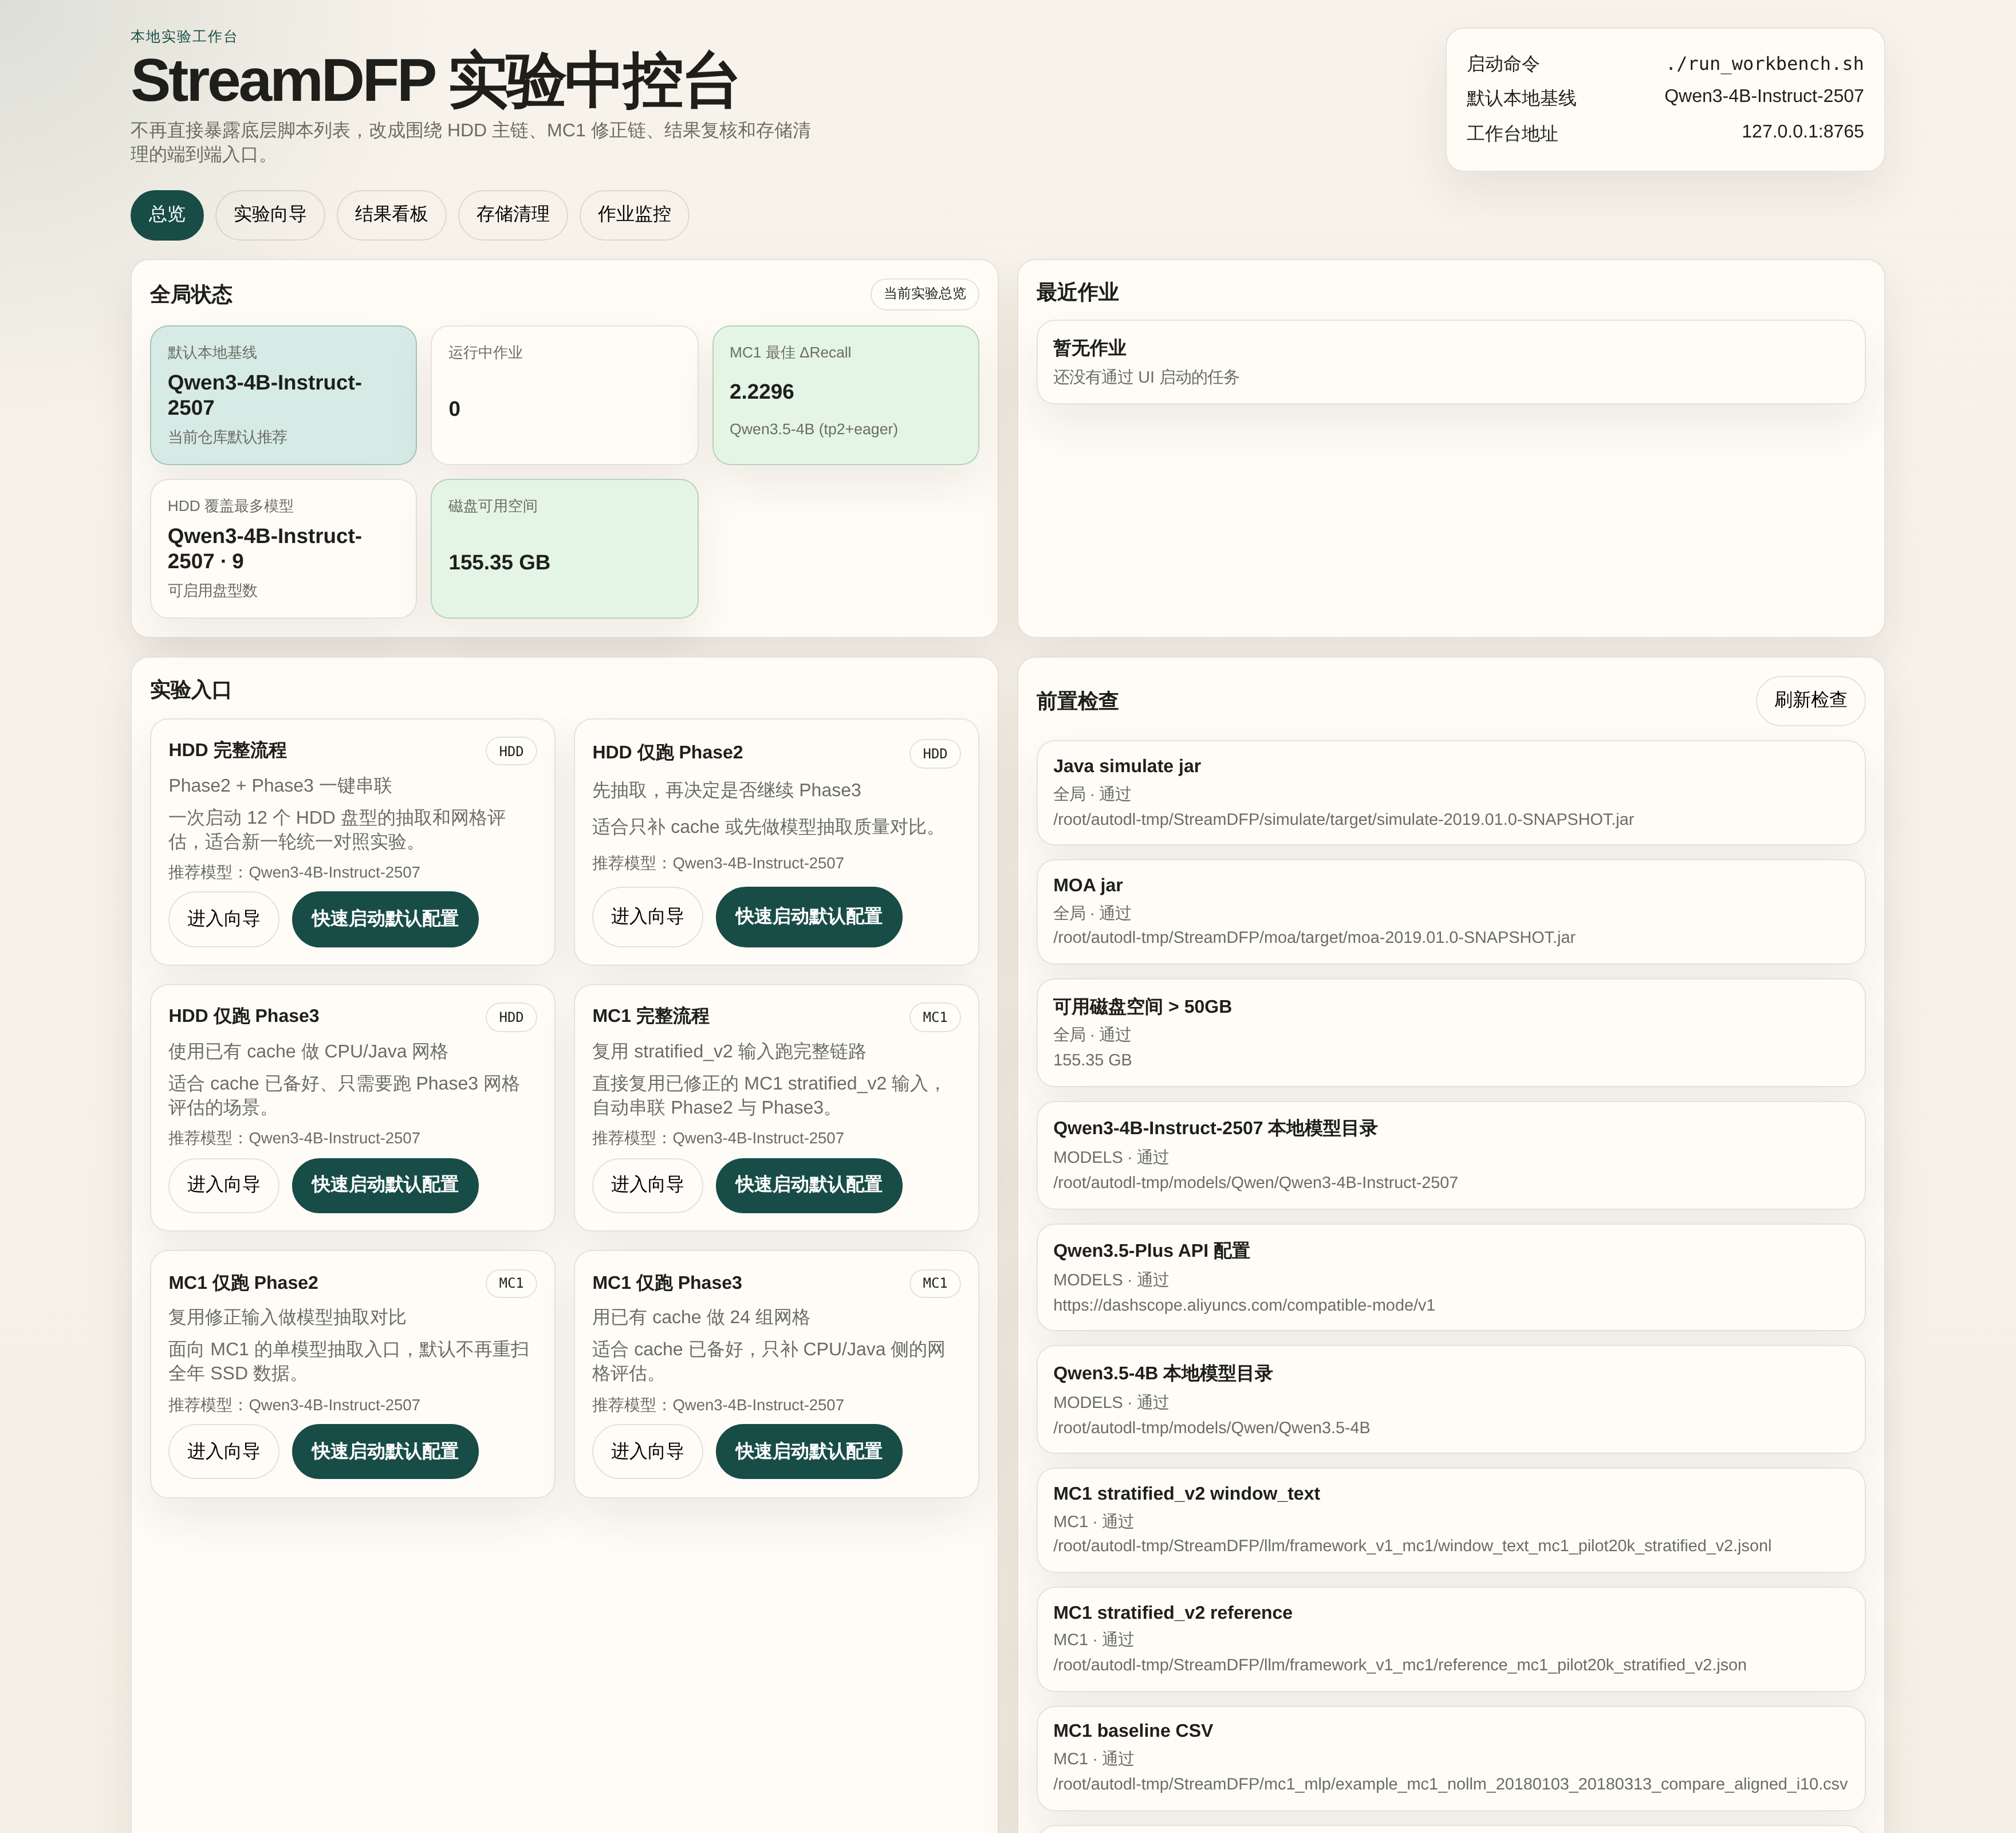
\includegraphics[width=0.78\textwidth,height=\textheight]{figures/fig_workbench_ui_overview_tall_20260410.png}
\caption{Workbench overview used for workflow selection, preflight
checking, and experiment monitoring.}
\end{figure}

\textbf{B. Representative Code Excerpts}

The main body argues for three implementation choices: rule-constrained
Phase 1 summarization, repaired stratified\_day\_disk sampling for mc1,
and gate-based Phase 3 cache filtering. The following abridged excerpts
are included to document those choices at the code level without
reproducing entire source files.

\textbf{B.1 Structured Phase 1 Summary Construction}

The following excerpt from \texttt{llm/window\_to\_text.py} illustrates
how a SMART window is converted into a constrained textual summary under
the \texttt{structured\_v2} schema.

\begin{Shaded}
\begin{Highlighting}[]
\CommentTok{\# excerpt from llm/window\_to\_text.py}
\NormalTok{root\_cause, scores }\OperatorTok{=}\NormalTok{ infer\_root\_cause(stats) }\ControlFlowTok{if}\NormalTok{ stats }\ControlFlowTok{else}\NormalTok{ (}
    \StringTok{"unknown"}\NormalTok{,}
\NormalTok{    \{k: }\FloatTok{0.0} \ControlFlowTok{for}\NormalTok{ k }\KeywordTok{in}\NormalTok{ ROOT\_CAUSES\},}
\NormalTok{)}
\NormalTok{selected }\OperatorTok{=}\NormalTok{ \_select\_summary\_features(stats, top\_k)}
\NormalTok{selected\_items: List[Dict] }\OperatorTok{=}\NormalTok{ []}
\ControlFlowTok{for}\NormalTok{ feat }\KeywordTok{in}\NormalTok{ selected:}
\NormalTok{    item }\OperatorTok{=}\NormalTok{ stats[feat]}
\NormalTok{    selected\_items.append(item)}

\NormalTok{rule\_score\_line }\OperatorTok{=}\NormalTok{ (}
    \StringTok{"RULE\_SCORE: "}
    \SpecialStringTok{f"media=}\SpecialCharTok{\{}\NormalTok{scores[}\StringTok{\textquotesingle{}media\textquotesingle{}}\NormalTok{]}\SpecialCharTok{:.3f\}}\SpecialStringTok{ "}
    \SpecialStringTok{f"interface=}\SpecialCharTok{\{}\NormalTok{scores[}\StringTok{\textquotesingle{}interface\textquotesingle{}}\NormalTok{]}\SpecialCharTok{:.3f\}}\SpecialStringTok{ "}
    \SpecialStringTok{f"temperature=}\SpecialCharTok{\{}\NormalTok{scores[}\StringTok{\textquotesingle{}temperature\textquotesingle{}}\NormalTok{]}\SpecialCharTok{:.3f\}}\SpecialStringTok{ "}
    \SpecialStringTok{f"power=}\SpecialCharTok{\{}\NormalTok{scores[}\StringTok{\textquotesingle{}power\textquotesingle{}}\NormalTok{]}\SpecialCharTok{:.3f\}}\SpecialStringTok{ "}
    \SpecialStringTok{f"workload=}\SpecialCharTok{\{}\NormalTok{scores[}\StringTok{\textquotesingle{}workload\textquotesingle{}}\NormalTok{]}\SpecialCharTok{:.3f\}}\SpecialStringTok{"}
\NormalTok{)}

\ControlFlowTok{if}\NormalTok{ summary\_schema }\OperatorTok{==} \StringTok{"structured\_v2"}\NormalTok{:}
\NormalTok{    lines }\OperatorTok{=}\NormalTok{ [}
        \SpecialStringTok{f"WINDOW: }\SpecialCharTok{\{}\NormalTok{start\_day}\SpecialCharTok{\}}\SpecialStringTok{\textasciitilde{}}\SpecialCharTok{\{}\NormalTok{end\_day}\SpecialCharTok{\}}\SpecialStringTok{ (}\SpecialCharTok{\{}\NormalTok{n\_rows}\SpecialCharTok{\}}\SpecialStringTok{d) disk=}\SpecialCharTok{\{}\NormalTok{\_mask\_disk\_id(disk\_id)}\SpecialCharTok{\}}\SpecialStringTok{"}\NormalTok{,}
\NormalTok{        \_format\_data\_quality\_line(stats, n\_rows),}
\NormalTok{        rule\_score\_line,}
\NormalTok{        \_format\_rule\_top2\_line(scores),}
\NormalTok{        \_format\_allowed\_event\_features\_line(selected\_items),}
\NormalTok{    ]}
\NormalTok{    lines.extend(\_format\_anomaly\_table\_lines(selected\_items, anomaly\_top\_k))}
\NormalTok{    lines.append(\_format\_cause\_evidence\_line(stats))}
\NormalTok{    lines.append(}\SpecialStringTok{f"RULE\_PRED: }\SpecialCharTok{\{}\NormalTok{root\_cause}\SpecialCharTok{\}}\SpecialStringTok{"}\NormalTok{)}
    \ControlFlowTok{if} \BuiltInTok{bool}\NormalTok{(ACTIVE\_SUMMARY.get(}\StringTok{"emit\_legacy\_text"}\NormalTok{, }\VariableTok{False}\NormalTok{)):}
\NormalTok{        lines.append(\_format\_persistence\_line(selected\_items))}
\NormalTok{        lines.append(\_format\_trend\_delta\_line(selected\_items))}
\NormalTok{        lines.append(\_format\_feature\_delta\_topk\_line(selected\_items))}
\NormalTok{        lines.append(\_format\_persistence\_profile\_line(selected\_items))}
\NormalTok{        lines.append(\_format\_burst\_vs\_drift\_line(selected\_items))}
\NormalTok{        lines.append(\_format\_group\_signal\_line(stats))}
    \ControlFlowTok{return} \StringTok{"}\CharTok{\textbackslash{}n}\StringTok{"}\NormalTok{.join(lines)}
\end{Highlighting}
\end{Shaded}

\textbf{B.2 Repaired stratified\_day\_disk Sampling}

The next excerpt documents the sampling logic used to repair the earlier
mc1 branch. Instead of truncating windows sequentially, the sampler
first allocates day-level quotas and then prefers under-represented
disks within each day.

\begin{Shaded}
\begin{Highlighting}[]
\CommentTok{\# excerpt from llm/window\_to\_text.py}
\ControlFlowTok{if}\NormalTok{ sample\_mode }\OperatorTok{!=} \StringTok{"stratified\_day\_disk"}\NormalTok{:}
    \ControlFlowTok{raise} \PreprocessorTok{ValueError}\NormalTok{(}\SpecialStringTok{f"Unsupported sample mode: }\SpecialCharTok{\{}\NormalTok{sample\_mode}\SpecialCharTok{\}}\SpecialStringTok{"}\NormalTok{)}

\NormalTok{day\_counts: Dict[}\BuiltInTok{str}\NormalTok{, }\BuiltInTok{int}\NormalTok{] }\OperatorTok{=}\NormalTok{ \{\}}
\ControlFlowTok{for}\NormalTok{ \_, day, \_, \_, \_, \_ }\KeywordTok{in}\NormalTok{ iter\_window\_records(}
\NormalTok{    data\_root,}
\NormalTok{    features,}
\NormalTok{    window\_days,}
\NormalTok{    date\_format,}
\NormalTok{    disk\_model,}
    \VariableTok{None}\NormalTok{,}
\NormalTok{    disk\_id\_prefix,}
\NormalTok{    output\_start\_date,}
\NormalTok{    output\_end\_date,}
\NormalTok{):}
\NormalTok{    day\_counts[day] }\OperatorTok{=}\NormalTok{ day\_counts.get(day, }\DecValTok{0}\NormalTok{) }\OperatorTok{+} \DecValTok{1}

\NormalTok{quotas }\OperatorTok{=}\NormalTok{ \_allocate\_day\_quotas(day\_counts, }\BuiltInTok{int}\NormalTok{(max\_windows), }\BuiltInTok{int}\NormalTok{(sample\_seed))}
\NormalTok{heaps: Dict[}\BuiltInTok{str}\NormalTok{, List[Tuple[}\BuiltInTok{float}\NormalTok{, Tuple[}\BuiltInTok{str}\NormalTok{, }\BuiltInTok{str}\NormalTok{, }\BuiltInTok{str}\NormalTok{, Dict[}\BuiltInTok{str}\NormalTok{, Dict], Dict, }\BuiltInTok{int}\NormalTok{]]]] }\OperatorTok{=}\NormalTok{ \{}
\NormalTok{    day: [] }\ControlFlowTok{for}\NormalTok{ day, quota }\KeywordTok{in}\NormalTok{ quotas.items() }\ControlFlowTok{if}\NormalTok{ quota }\OperatorTok{\textgreater{}} \DecValTok{0}
\NormalTok{\}}
\NormalTok{seen\_per\_day\_disk: Dict[Tuple[}\BuiltInTok{str}\NormalTok{, }\BuiltInTok{str}\NormalTok{], }\BuiltInTok{int}\NormalTok{] }\OperatorTok{=}\NormalTok{ \{\}}
\NormalTok{rng }\OperatorTok{=}\NormalTok{ random.Random(}\BuiltInTok{int}\NormalTok{(sample\_seed))}

\ControlFlowTok{for}\NormalTok{ rec }\KeywordTok{in}\NormalTok{ iter\_window\_records(}
\NormalTok{    data\_root,}
\NormalTok{    features,}
\NormalTok{    window\_days,}
\NormalTok{    date\_format,}
\NormalTok{    disk\_model,}
    \VariableTok{None}\NormalTok{,}
\NormalTok{    disk\_id\_prefix,}
\NormalTok{    output\_start\_date,}
\NormalTok{    output\_end\_date,}
\NormalTok{):}
\NormalTok{    disk\_id, day, }\OperatorTok{*}\NormalTok{\_ }\OperatorTok{=}\NormalTok{ rec}
\NormalTok{    quota }\OperatorTok{=}\NormalTok{ quotas.get(day, }\DecValTok{0}\NormalTok{)}
    \ControlFlowTok{if}\NormalTok{ quota }\OperatorTok{\textless{}=} \DecValTok{0}\NormalTok{:}
        \ControlFlowTok{continue}

\NormalTok{    key }\OperatorTok{=}\NormalTok{ (day, disk\_id)}
\NormalTok{    seen }\OperatorTok{=}\NormalTok{ seen\_per\_day\_disk.get(key, }\DecValTok{0}\NormalTok{) }\OperatorTok{+} \DecValTok{1}
\NormalTok{    seen\_per\_day\_disk[key] }\OperatorTok{=}\NormalTok{ seen}

    \CommentTok{\# prefer rare disks within each day while keeping randomness}
\NormalTok{    weight }\OperatorTok{=} \FloatTok{1.0} \OperatorTok{/}\NormalTok{ math.sqrt(}\BuiltInTok{float}\NormalTok{(seen))}
\NormalTok{    priority }\OperatorTok{=}\NormalTok{ rng.random() }\OperatorTok{**}\NormalTok{ (}\FloatTok{1.0} \OperatorTok{/} \BuiltInTok{max}\NormalTok{(weight, }\FloatTok{1e{-}6}\NormalTok{))}
\NormalTok{    heap }\OperatorTok{=}\NormalTok{ heaps[day]}
\NormalTok{    item }\OperatorTok{=}\NormalTok{ (priority, rec)}
    \ControlFlowTok{if} \BuiltInTok{len}\NormalTok{(heap) }\OperatorTok{\textless{}}\NormalTok{ quota:}
\NormalTok{        heapq.heappush(heap, item)}
    \ControlFlowTok{elif}\NormalTok{ priority }\OperatorTok{\textgreater{}}\NormalTok{ heap[}\DecValTok{0}\NormalTok{][}\DecValTok{0}\NormalTok{]:}
\NormalTok{        heapq.heapreplace(heap, item)}

\NormalTok{selected }\OperatorTok{=}\NormalTok{ []}
\ControlFlowTok{for}\NormalTok{ day }\KeywordTok{in} \BuiltInTok{sorted}\NormalTok{(heaps.keys()):}
\NormalTok{    day\_records }\OperatorTok{=}\NormalTok{ [it[}\DecValTok{1}\NormalTok{] }\ControlFlowTok{for}\NormalTok{ it }\KeywordTok{in}\NormalTok{ heaps[day]]}
\NormalTok{    day\_records.sort(key}\OperatorTok{=}\KeywordTok{lambda}\NormalTok{ x: (x[}\DecValTok{1}\NormalTok{], x[}\DecValTok{0}\NormalTok{]))}
\NormalTok{    selected.extend(day\_records)}
\end{Highlighting}
\end{Shaded}

\textbf{B.3 Gate-Based Cache Variant Construction}

The final excerpt from \texttt{llm/scripts/build\_cache\_variant.py}
shows how the LLM cache is filtered before reinjection into the
downstream predictor. Windows can be rejected because they are
\texttt{unknown}, fail the quality gate, disagree with the top
rule-based cause, or have insufficient retained event severity.

\begin{Shaded}
\begin{Highlighting}[]
\CommentTok{\# excerpt from llm/scripts/build\_cache\_variant.py}
\NormalTok{rule\_top }\OperatorTok{=}\NormalTok{ \_load\_rule\_top\_map(window\_text\_path) }\ControlFlowTok{if}\NormalTok{ require\_rule\_match }\ControlFlowTok{else}\NormalTok{ \{\}}
\NormalTok{keep\_dims\_ordered }\OperatorTok{=}\NormalTok{ \_dedupe\_keep\_order(DEFAULT\_META\_DIMS }\OperatorTok{+}\NormalTok{ keep\_events)}
\NormalTok{keep\_dims }\OperatorTok{=} \BuiltInTok{set}\NormalTok{(keep\_dims\_ordered)}

\ControlFlowTok{for}\NormalTok{ line }\KeywordTok{in}\NormalTok{ fr:}
\NormalTok{    row }\OperatorTok{=}\NormalTok{ json.loads(line)}
\NormalTok{    root\_cause }\OperatorTok{=} \BuiltInTok{str}\NormalTok{(}
\NormalTok{        row.get(root\_cause\_field, row.get(}\StringTok{"root\_cause"}\NormalTok{, }\StringTok{"unknown"}\NormalTok{))}
\NormalTok{    ).strip().lower()}
\NormalTok{    risk\_hint }\OperatorTok{=}\NormalTok{ \_safe\_float(row.get(}\StringTok{"risk\_hint"}\NormalTok{), }\FloatTok{0.0}\NormalTok{)}
\NormalTok{    confidence }\OperatorTok{=}\NormalTok{ \_safe\_float(row.get(}\StringTok{"confidence"}\NormalTok{), }\FloatTok{0.0}\NormalTok{)}
\NormalTok{    label\_noise }\OperatorTok{=}\NormalTok{ \_safe\_float(row.get(}\StringTok{"label\_noise\_risk"}\NormalTok{), }\FloatTok{0.0}\NormalTok{)}
\NormalTok{    q }\OperatorTok{=} \BuiltInTok{min}\NormalTok{(confidence, risk\_hint) }\OperatorTok{*}\NormalTok{ (}\FloatTok{1.0} \OperatorTok{{-}} \BuiltInTok{max}\NormalTok{(}\FloatTok{0.0}\NormalTok{, }\BuiltInTok{min}\NormalTok{(}\FloatTok{1.0}\NormalTok{, label\_noise)))}

\NormalTok{    keep }\OperatorTok{=} \VariableTok{True}
    \ControlFlowTok{if}\NormalTok{ root\_cause }\OperatorTok{==} \StringTok{"unknown"}\NormalTok{:}
\NormalTok{        keep }\OperatorTok{=} \VariableTok{False}
\NormalTok{        drop\_unknown }\OperatorTok{+=} \DecValTok{1}
    \ControlFlowTok{elif}\NormalTok{ q }\OperatorTok{\textless{}}\NormalTok{ q\_gate:}
\NormalTok{        keep }\OperatorTok{=} \VariableTok{False}
\NormalTok{        drop\_q }\OperatorTok{+=} \DecValTok{1}

    \ControlFlowTok{if}\NormalTok{ keep }\KeywordTok{and}\NormalTok{ require\_rule\_match:}
\NormalTok{        disk\_id }\OperatorTok{=} \BuiltInTok{str}\NormalTok{(row.get(}\StringTok{"disk\_id"}\NormalTok{, }\StringTok{""}\NormalTok{))}
\NormalTok{        day }\OperatorTok{=} \BuiltInTok{str}\NormalTok{(row.get(}\StringTok{"window\_end\_time"}\NormalTok{, }\StringTok{""}\NormalTok{))}
\NormalTok{        top }\OperatorTok{=}\NormalTok{ rule\_top.get((disk\_id, day))}
        \ControlFlowTok{if}\NormalTok{ top }\KeywordTok{is} \VariableTok{None}\NormalTok{:}
\NormalTok{            keep }\OperatorTok{=} \VariableTok{False}
\NormalTok{            drop\_rule }\OperatorTok{+=} \DecValTok{1}
\NormalTok{            missing\_rule\_key }\OperatorTok{+=} \DecValTok{1}
        \ControlFlowTok{elif}\NormalTok{ root\_cause }\OperatorTok{!=}\NormalTok{ top:}
\NormalTok{            keep }\OperatorTok{=} \VariableTok{False}
\NormalTok{            drop\_rule }\OperatorTok{+=} \DecValTok{1}

    \ControlFlowTok{if}\NormalTok{ keep:}
\NormalTok{        sev\_sum }\OperatorTok{=} \FloatTok{0.0}
        \ControlFlowTok{for}\NormalTok{ d }\KeywordTok{in}\NormalTok{ keep\_events:}
\NormalTok{            sev\_sum }\OperatorTok{+=}\NormalTok{ \_safe\_float(row.get(}\SpecialStringTok{f"z\_llm\_}\SpecialCharTok{\{d\}}\SpecialStringTok{"}\NormalTok{), }\FloatTok{0.0}\NormalTok{)}
        \ControlFlowTok{if}\NormalTok{ sev\_sum }\OperatorTok{\textless{}}\NormalTok{ sev\_sum\_gate:}
\NormalTok{            keep }\OperatorTok{=} \VariableTok{False}
\NormalTok{            drop\_sev }\OperatorTok{+=} \DecValTok{1}

    \ControlFlowTok{for}\NormalTok{ idx }\KeywordTok{in} \BuiltInTok{range}\NormalTok{(dim\_bound):}
\NormalTok{        key }\OperatorTok{=} \SpecialStringTok{f"z\_llm\_}\SpecialCharTok{\{}\NormalTok{idx}\SpecialCharTok{\}}\SpecialStringTok{"}
        \ControlFlowTok{if}\NormalTok{ keep }\KeywordTok{and}\NormalTok{ idx }\KeywordTok{in}\NormalTok{ keep\_dims:}
\NormalTok{            row[key] }\OperatorTok{=}\NormalTok{ \_safe\_float(row.get(key), }\FloatTok{0.0}\NormalTok{)}
        \ControlFlowTok{else}\NormalTok{:}
\NormalTok{            row[key] }\OperatorTok{=} \FloatTok{0.0}
\end{Highlighting}
\end{Shaded}


\end{document}
